\chapter{Event selection}
\label{select}

The data reported in this analysis were taken during the e1e run periods in the Hall B during November 2002 - January 2003 that included several configurations (hydrogen and deuterium targets as well as two different beam energies of 1 GeV and 2.039 GeV). The torus current was 2250~A and the mini torus current 5995~A. This particular analysis is concentrated on the data obtained with the 2 cm long liquid hydrogen target located at -0.2 cm along z-axis, a 2.039 GeV polarized electron beam, and the CLAS detector. The run numbers' range of this experimental setup is 36118 - 36512. There is a gap in the run numbering between runs 36160 and 36387, which coincides with Christmas and New Year of 2002-2003 and is most likely connected to a database server glitch (there are no entries in the database nor files on the silo associated with run numbers in this gap). Totally about 1.5 billion triggers over a month of a beamtime were accumulated.
The  list of full and empty target runs that are used in the analysis is presented in Tab.~\ref{tab_good_runs}.

\begin{table}[htp]
\centering 




\begin{tabular}{|c|c|}

\hline
Full target runs & Empty target runs\\
\hline 
36117--36122, 36125--36129, 36133--36142 & 35124  \\
36144, 36145, 36147--36150, 36152--36154 & 36428  \\
36156, 36158--36160, 36429--36434 & 36495  \\ 
36437,  36441--36447, 36449, 36450 & \\
36452--36454, 36458--36467, 36469 & \\
36473--36478, 36480--36482, 36484--36492 & \\
36497--36503, 36505--36511 & \\
\hline 
\end{tabular}
\caption{\small List of the runs that are used in the analysis. \label{tab_good_runs}}
\end{table}

\section{Particles identification}
\label{ident}

In this analysis the first in time particle that gives signals in all four parts of the CLAS detector is chosen as electron candidate for each event. To identify hadrons only signals in drift chambers and time-of-flight system are required.

All data accumulated during the run is stored in BOS~\cite{BOS:bank} files. For all events selected for analysis the number of geometrically reconstructed particles ($gpart$) was required to be greater than zero. The $gpart$ variable is extracted from variable $NPGP$ in HEVT bank according to~\ref{eq:id_gpart}. 

\begin{equation}
NPGP=(\text{Number of final reconstructed particles})\times100 + gpart
\label{eq:id_gpart}
\end{equation}

One more requirement is that the status word ($stat$) is greater than zero (variable $Status$ in EVNT bank).

Then, as mentioned above, for electron candidates signals in all four detectors are required (all variables $DCStat$, $CCStat$, $SCStat$, $ECStat$ from EVNT bank must be greater than zero). For hadrons only the variables $DCStat$ and $SCStat$ from EVNT bank are required to be greater than zero. 

Finally the corresponding charge for all particle candidates (variable $Charge$ from EVNT bank) is required to be plus or minus one depending on the particle candidate's type.
 

\subsection{Electron identification}
\label{electron} 

Firstly electromagnetic calorimeter (EC) and \v Cerenkov counter (CC) responses need to be checked, to select good electrons from the electron candidates.

\subsubsection{EC cuts}
\label{ec_cuts}


On the hardware level the calorimeter threshold was set
to cut off events as close as possible to the kinematic edges
of the $W$ and $Q^{2}$ domain covered by the measurement, but far
enough to keep the low energy contamination within reasonable
limits. To select good electrons more precisely an additional calorimeter threshold cut on the software level  is applied. This cut accounts for the minimal momentum of the scattered electron that can be reconstructed ($P_{e'} > 0.461$~GeV) and is chosen according to~\cite{Egian:007}.

Then an additional cut (the so-called sampling fraction cut) was applied to  eliminate in part pion contamination. To develop this cut the fact that electrons and pions
have different  energy deposition patterns in EC was used. An electron produces an electromagnetic shower, where the
deposited energy is proportional to the electron momentum, while a $\pi^{-}$ as  minimum ionizing particle loses a constant
amount of energy per scintillator (2~MeV/cm) independently of its momentum. In Fig.~\ref{fig:ec_cut_data} total energy deposited in EC divided by the particle momentum is shown as function of particle momentum. The six plots represent six CLAS sectors. Events between the red curves are selected as good electron candidates for further analysis. The vertical red line at $P_{e'} = 0.461$~GeV shows EC threshold cut. The upper and lower red curves are obtained in the following way:  x-slices of 2D histograms are fit by Gaussians. In this way points that correspond to the positions of the fit maxima $\pm 3\sigma$ are obtained. These points determine the upper and lower boundaries for the cut. Finally, to obtain smooth curves, all points are fit by a second order polynom.  

\begin{figure}[htp]
\begin{center}
\framebox{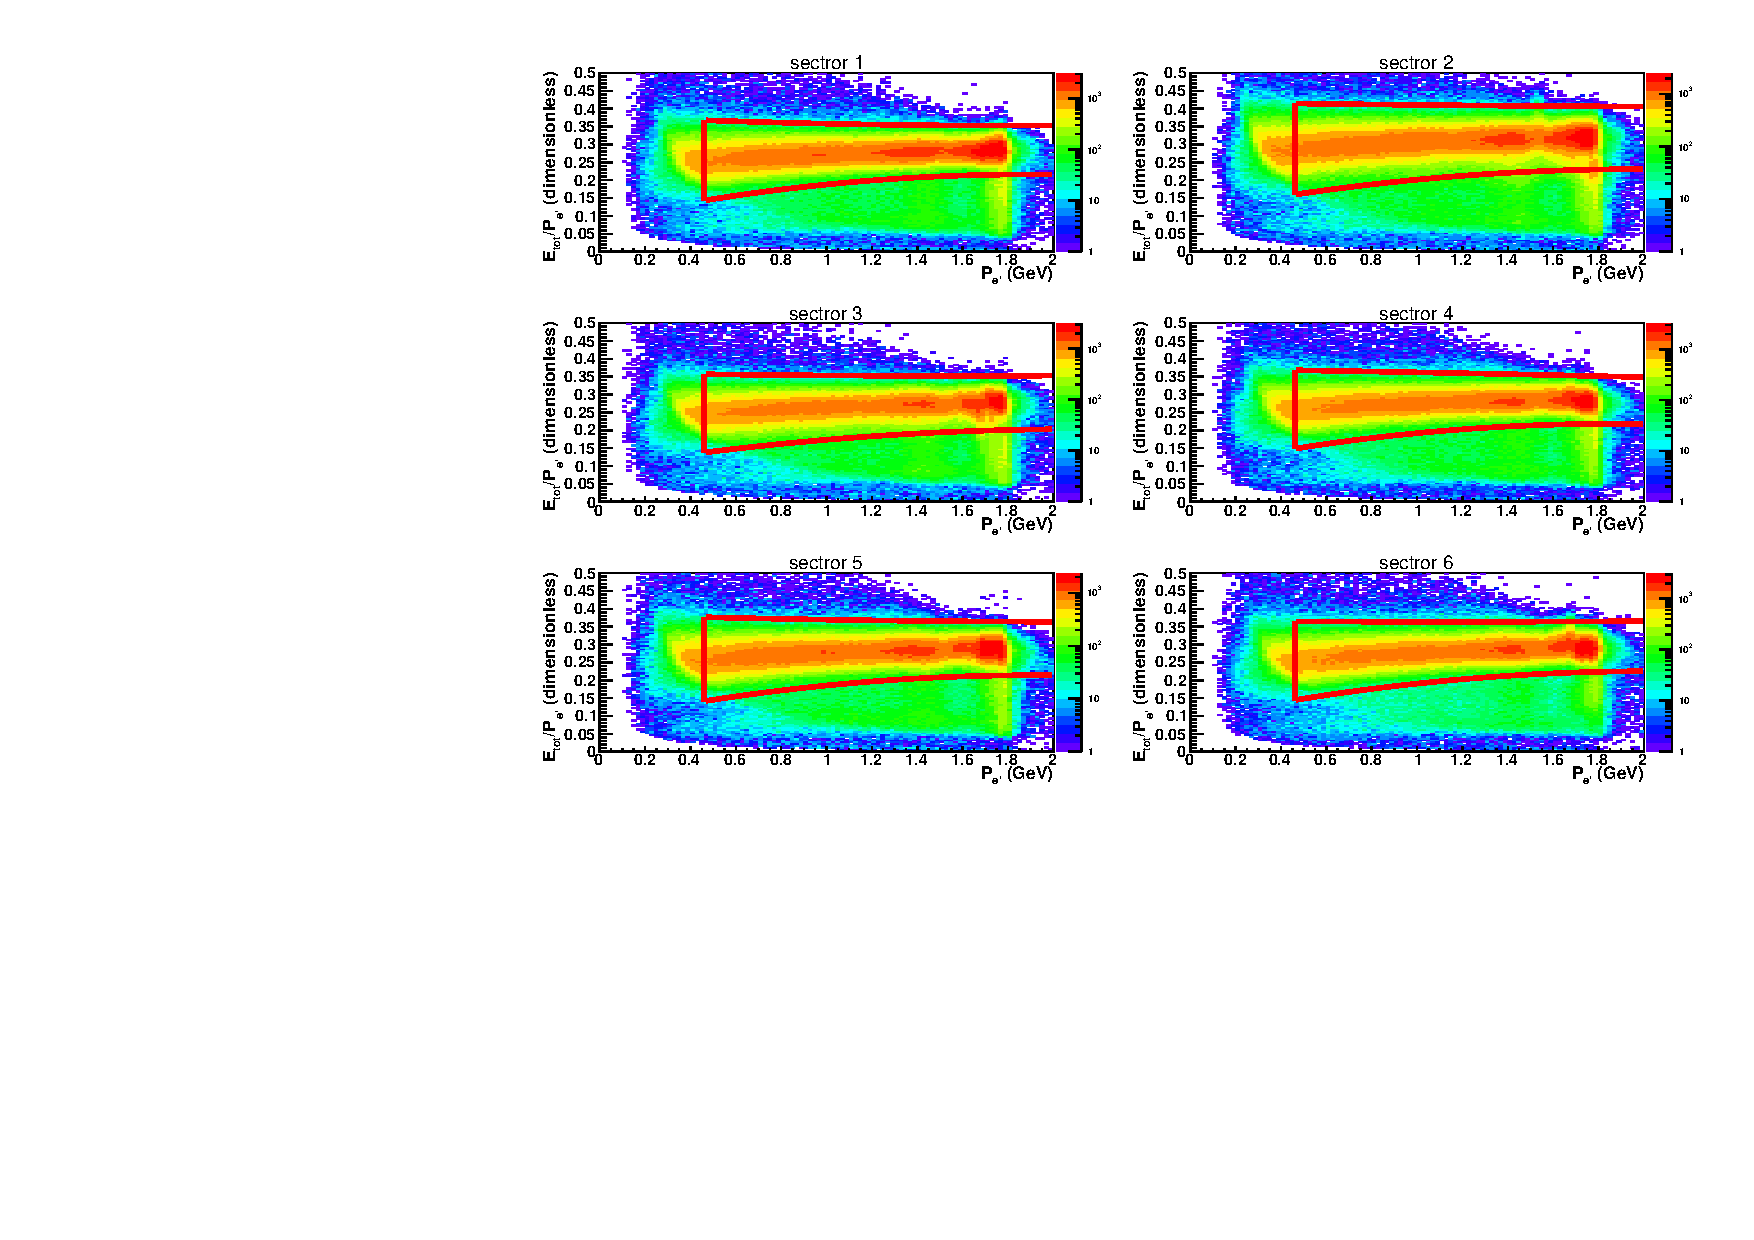
\includegraphics[width=12cm]{pictures/event_selection/ec_cut/ec_cut_data.pdf}}
\caption{\small Sampling fraction distributions for the data. Six plots correspond to six CLAS sectors. Events between red curves are selected for further analysis.} \label{fig:ec_cut_data}
\end{center}
\end{figure}

\begin{figure}[htp]
\begin{center}
\framebox{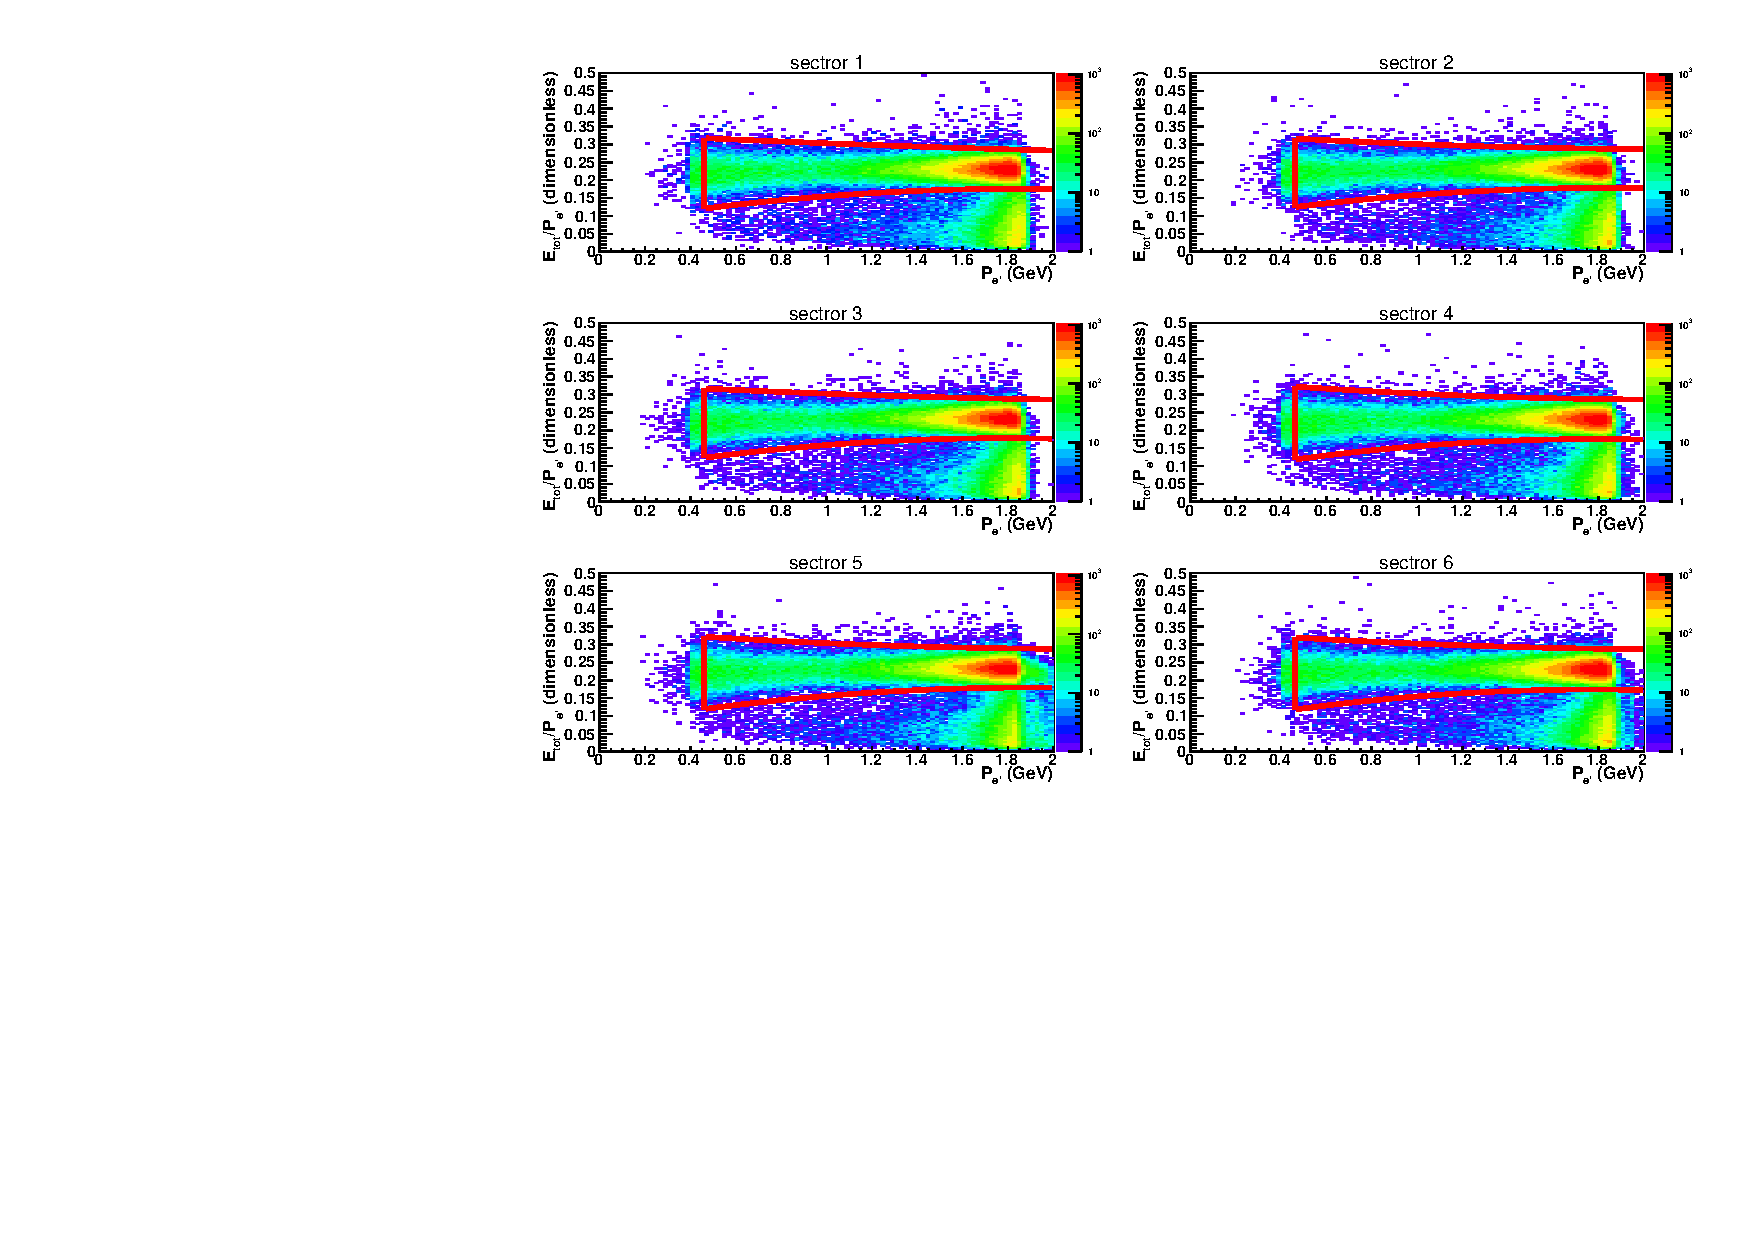
\includegraphics[width=12cm]{pictures/event_selection/ec_cut/ec_cut_sim.pdf}}
\caption{\small  Sampling fraction distributions for Monte Carlo. Six plots correspond to six CLAS sectors. Events between red curves are selected for further analysis.} \label{fig:ec_cut_sim}
\end{center}
\end{figure}

Both cuts on minimal electron energy and on sampling fraction are applied
both to experimental and Monte Carlo events. Since the Monte Carlo simulation does not reproduce electromagnetic showers good enough, the sampling fraction cuts for the simulation, obtained using the same procedure as for the data, look slightly different (see Fig.~\ref{fig:ec_cut_sim}).

In Fig.~\ref{fig_eout_ein} the energy deposited in the outer part of EC versus the energy deposited in the inner part of EC is shown before (left plot) and after (right plot) final electron identification. As it is seen in this plot the spot in the left bottom corner that corresponds to the pion contamination disappears that verifies the reliability of the electron selection.

\begin{figure}
\begin{center} 
\framebox{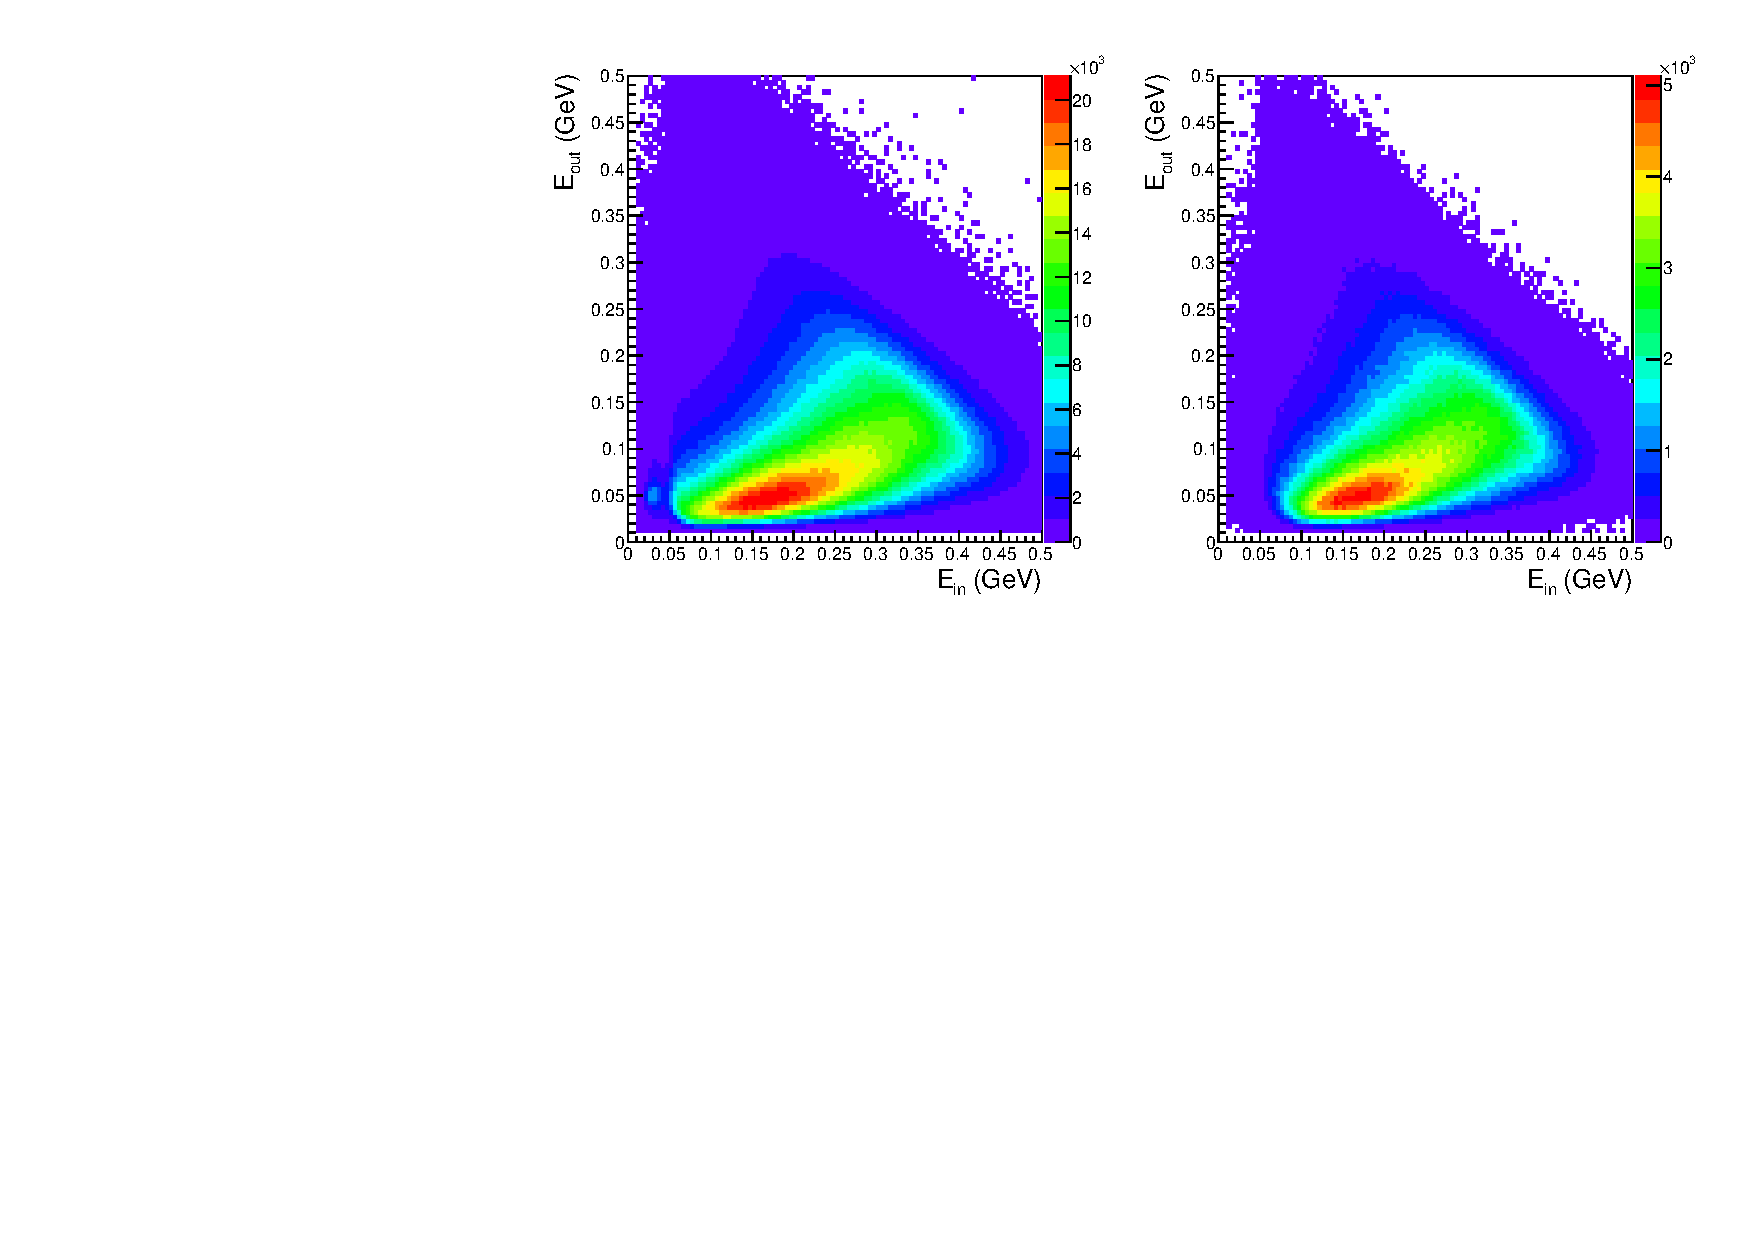
\includegraphics[width=12cm]{pictures/event_selection/ec_cut/eout_vs_ein.pdf}}
\caption{\small Energy deposited in the outer part of EC versus energy deposited in the inner part of EC before (left plot) and after (right plot) final electron selection. \label{fig_eout_ein}} 
\end{center}
\end{figure}

 

\subsubsection{CC cuts}
\label{cc_cuts} 

To improve the quality of electron candidate selection and $\pi^{-}/e^{-}$ separation a \v Cerenkov counter is used. In this experiment the \v Cerenkov counter had inhomogeneously distributed zones with partially low detection efficiency. For that purpose a geometrical cut for the removal of CC low efficiency zones is established. This cut is defined in the plane of \v Cerenkov counter. 
Since polar and azimuthal angles $(\theta_{cc},\varphi_{cc})$ in the CC plane are not directly defined in the BOS banks~\cite{BOS:bank} some calculations were made to derive these angles from variables available in DCPB bank. Fig.~\ref{fig:cc_plane_def} illustrates these calculations.

\begin{figure}[htp]
\begin{center}
\framebox{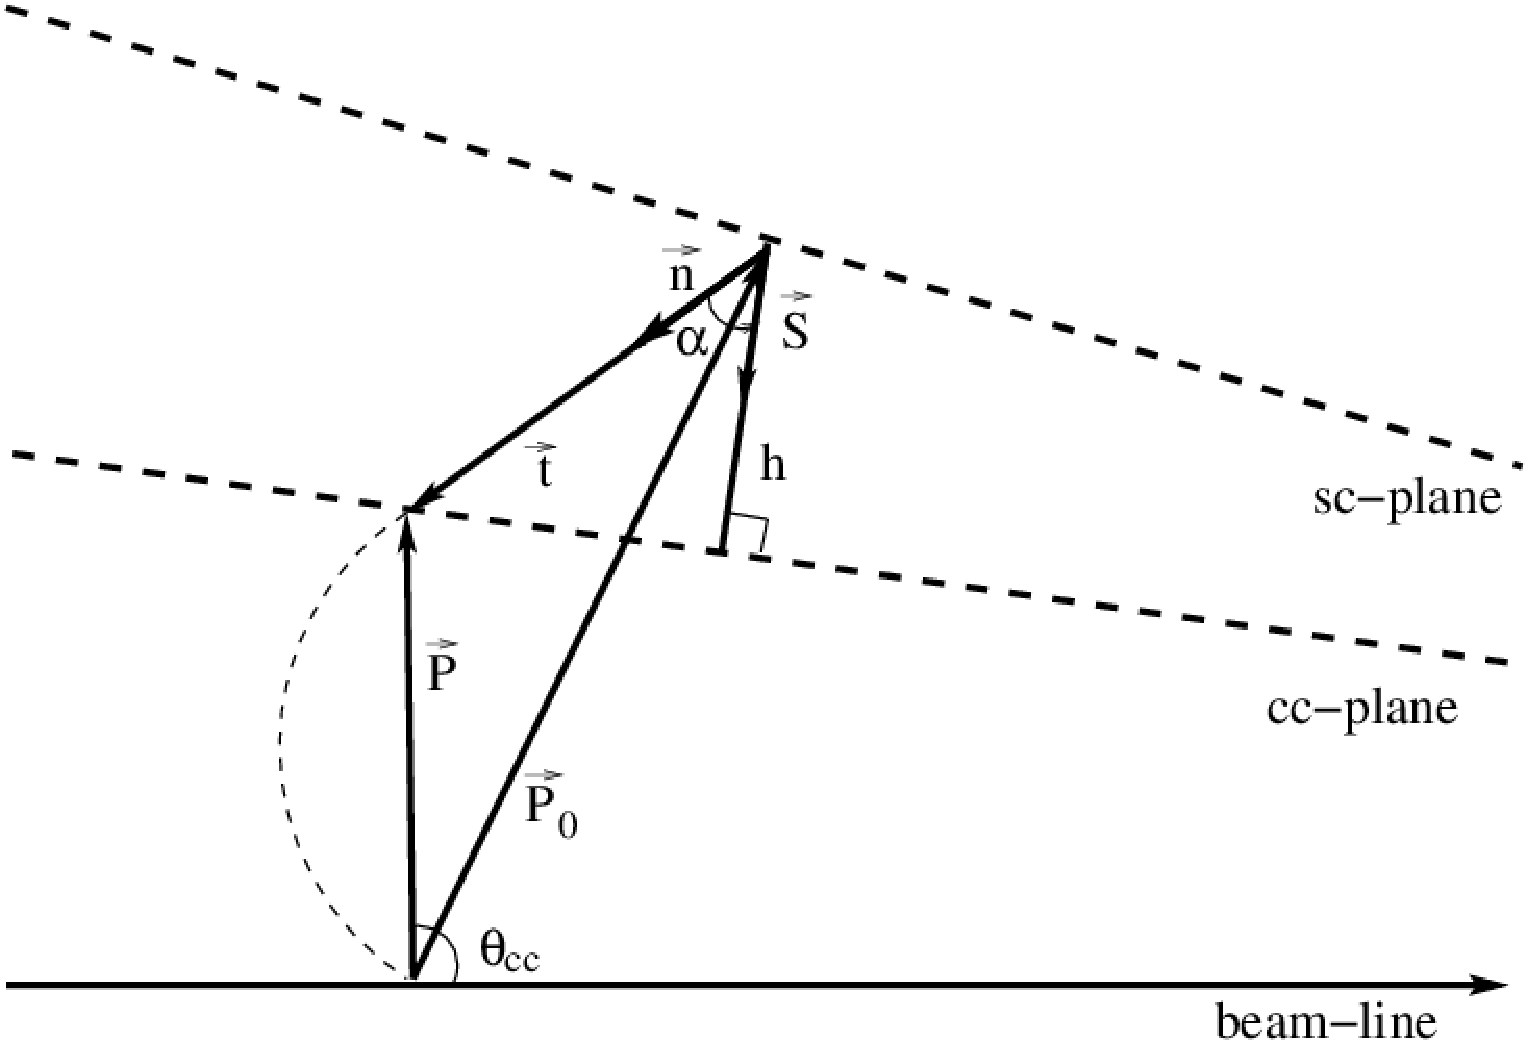
\includegraphics[width=7cm]{pictures/event_selection/cc_cut/cc_plane_def.pdf}}
\caption{\small  Calculation of polar $\theta_{cc}$ and azimuthal $\varphi_{cc}$  angles in the CC plane using variables that are available in DCPB bank.} \label{fig:cc_plane_def}
\end{center}
\end{figure}

 
The equation~\ref{eq:cc_plane} of the CC plane is known from~\cite{Osipenko:2004}: 

\begin{equation}
\begin{aligned}
 Ax+By+Cz+D = 0,  \\ \label{eq:cc_plane}
  D=1.,  \\ 
  A=-0.000785, \\ 
  B=0,  \\
  C=-0.00168, \\
  \overrightarrow{S} = (A,B,C)
\end{aligned}  
\end{equation}
The distance ($h$) from the SC hit point to the CC plane (see Fig.~\ref{fig:cc_plane_def}) is then given by

\begin{equation}
h=\frac{(\overrightarrow{S} \cdot \overrightarrow{P_{0}})+D}{\left |\overrightarrow{S}  \right |},
\label{eq:cc_h_distance}
\end{equation}
where components of $\overrightarrow{P_{0}}$ are available in  DCPB bank ($x\_sc, y\_sc, z\_sc$). 
 A tangent to the particle track (the track is shown by a dashed line in~Fig.~\ref{fig:cc_plane_def})  at the point of intersection with the CC plane ($ \vec t$) can be written as 
\begin{equation}
\left | \overrightarrow{t} \right |=\frac{h}{cos(\alpha )}.
\label{eq:cc_t_vec} 
\end{equation}
In turn $cos(\alpha )$ can be calculated as~\ref{eq:cc_cos_alpha}.
\begin{equation}
cos(\alpha )=\frac{(\overrightarrow{n} \cdot \overrightarrow{S})}{\left | \overrightarrow{S} \right |},
\label{eq:cc_cos_alpha} 
\end{equation}
 where $ \vec n$ is a unit vector in $ \vec t$-direction based on the DCPB bank variables ($cx\_sc, cy\_sc, cz\_sc$). It needs to be mentioned that there is no magnetic field between the CC and SC planes, so after hitting the CC plane the particle moves along the $ \vec t$-vector.






It is easy to see in Fig.~\ref{fig:cc_plane_def} that the vector $\overrightarrow{P}$, which goes from the  interaction vertex to the track intersection with the CC plane, is $\overrightarrow{P}=\overrightarrow{P_{0}}+\overrightarrow{t}$. Therefore, the angles $\theta_{cc}$ and $\varphi_{cc}$ can be calculated by~\ref{eq:cc_theta} and~\ref{eq:phi_theta}, respectively.


\begin{equation}
 \theta_{cc}=arccos\left ( \frac{P_z}{\left | \overrightarrow{P} \right |}\right )
\label{eq:cc_theta} 
\end{equation}

\begin{equation}
\begin{aligned}
\varphi_{cc} & = & arctan\left ( \frac{P_{y}}{P_{x}} \right ) \, \, \, \, \, \,\, \, \, \, \, \, \, \, \, \, \, \, & if & \, \, \,  P_{x}>0,\, \, \, P_{y}>0 & \\
\varphi_{cc} & = & arctan\left ( \frac{P_{y}}{P_{x}} \right )+2\pi  \, \, \,  & if & \, \, \,  P_{x}>0,\, \, \, P_{y}<0 & \\
\varphi_{cc} & = & arctan\left ( \frac{P_{y}}{P_{x}} \right )+\pi  \, \, \, &  if & \, \, \,  P_{x}<0,\, \, \, P_{y}<0 & \\
\varphi_{cc} & = & arctan\left ( \frac{P_{y}}{P_{x}} \right )+\pi  \, \, \, &  if & \, \, \,  P_{x}<0,\, \, \, P_{y}>0 & \\
\varphi_{cc} & = & \frac{\pi }{2} \, \, \,  \, \, \,  \, \, \, \, \, \,   \, \, \,  \, \, \, \, \, \,& if & \, \, \,  P_{x}=0,\, \, \, P_{y}>0 & \\
\varphi_{cc} & = & \frac{3\pi }{2} \, \, \,  \, \, \, \, \, \,   \, \, \,  \, \, \, \, \, \,&  if & \, \, \,  P_{x}=0,\, \, \, P_{y}<0 & \\
\label{eq:phi_theta} 
\end{aligned}
\end{equation}

%Segment from CCPB bank: segment = (status\%1000)/10. PMT from CCPB: pmt = (status/1000)-1.\\

%$\Delta T=T_{cc} +t/c-T_{sc}$

After the angles in the CC plane are defined, distributions $\varphi_{cc}$ vs. $\theta_{cc}$ are plotted for each CLAS sector (see Fig.~\ref{fig:ph_vs_th_cc}).
The quantity~\ref{eq:cc_ratio} is shown by the color code in Fig.~\ref{fig:ph_vs_th_cc}. This quantity varies from zero to one and shows the portion of good electrons with number of photoelectrons greater than five inside a $(\theta_{cc},\varphi_{cc})$ bin. Or in other words how efficient CC is in a given $(\theta_{cc},\varphi_{cc})$ bin. 
\begin{equation}
\frac{number\,\, of\,\, events\,\,  inside\,\, (\theta_{cc},\varphi_{cc})\,\, bin\,\, with\,\, more\,\, than\,\, 5\,\, photoelectrons\,\, in\,\, CC}{total\,\, number\,\, of\,\, events\,\,  inside\,\, (\theta_{cc},\varphi_{cc})\,\, bin}
\label{eq:cc_ratio}
\end{equation}
The edges of the distributions in Fig.~\ref{fig:ph_vs_th_cc} are sharp due to the fiducial cut that is applied in the CC plane~\ref{eq:cc_fiduch}. 
The shape of this cut  is taken from~\cite{Khetarpal:2010}.
\begin{equation}
\begin{aligned}
\theta_{cc} > 7.0+0.0032\varphi_{cc}+0.0499\varphi_{cc}^{2} \\
\left( \frac{\theta_{cc}-45.5^{o}}{34.5^{o}} \right)^{2} + \left( \frac{\varphi_{cc}}{21^{o}} \right)^{2} \le 1 \\
\left( \frac{\theta_{cc}-45.5^{o}}{1.75^{o}} \right)^{2} + \left( \frac{\varphi_{cc}}{21^{o}} \right)^{2} > 1 \\
\theta_{cc} < 45^{o} \, \, \,  \, \, \, \, \, \,   \, \, \,  \, \, \, \, \, \,
\label{eq:cc_fiduch}
\end{aligned}
\end{equation}
The two stripes in sector five in Fig.~\ref{fig:ph_vs_th_cc} correspond to the inefficient zones that will be discussed in~Sec.~\ref{fiduc}.

For further analysis only zones with a ratio~\ref{eq:cc_ratio} greater than $0.8$ are selected. These zones are shown in black in Fig.~\ref{fig:ph_vs_th_cc_08cut}. As it is seen in Fig.~\ref{fig:ph_vs_th_cc_08cut}, there is an inefficient zone in the middle of each sector, that is expected since two CC mirrors are joined there.

\begin{figure}[htp]
\begin{center}
\framebox{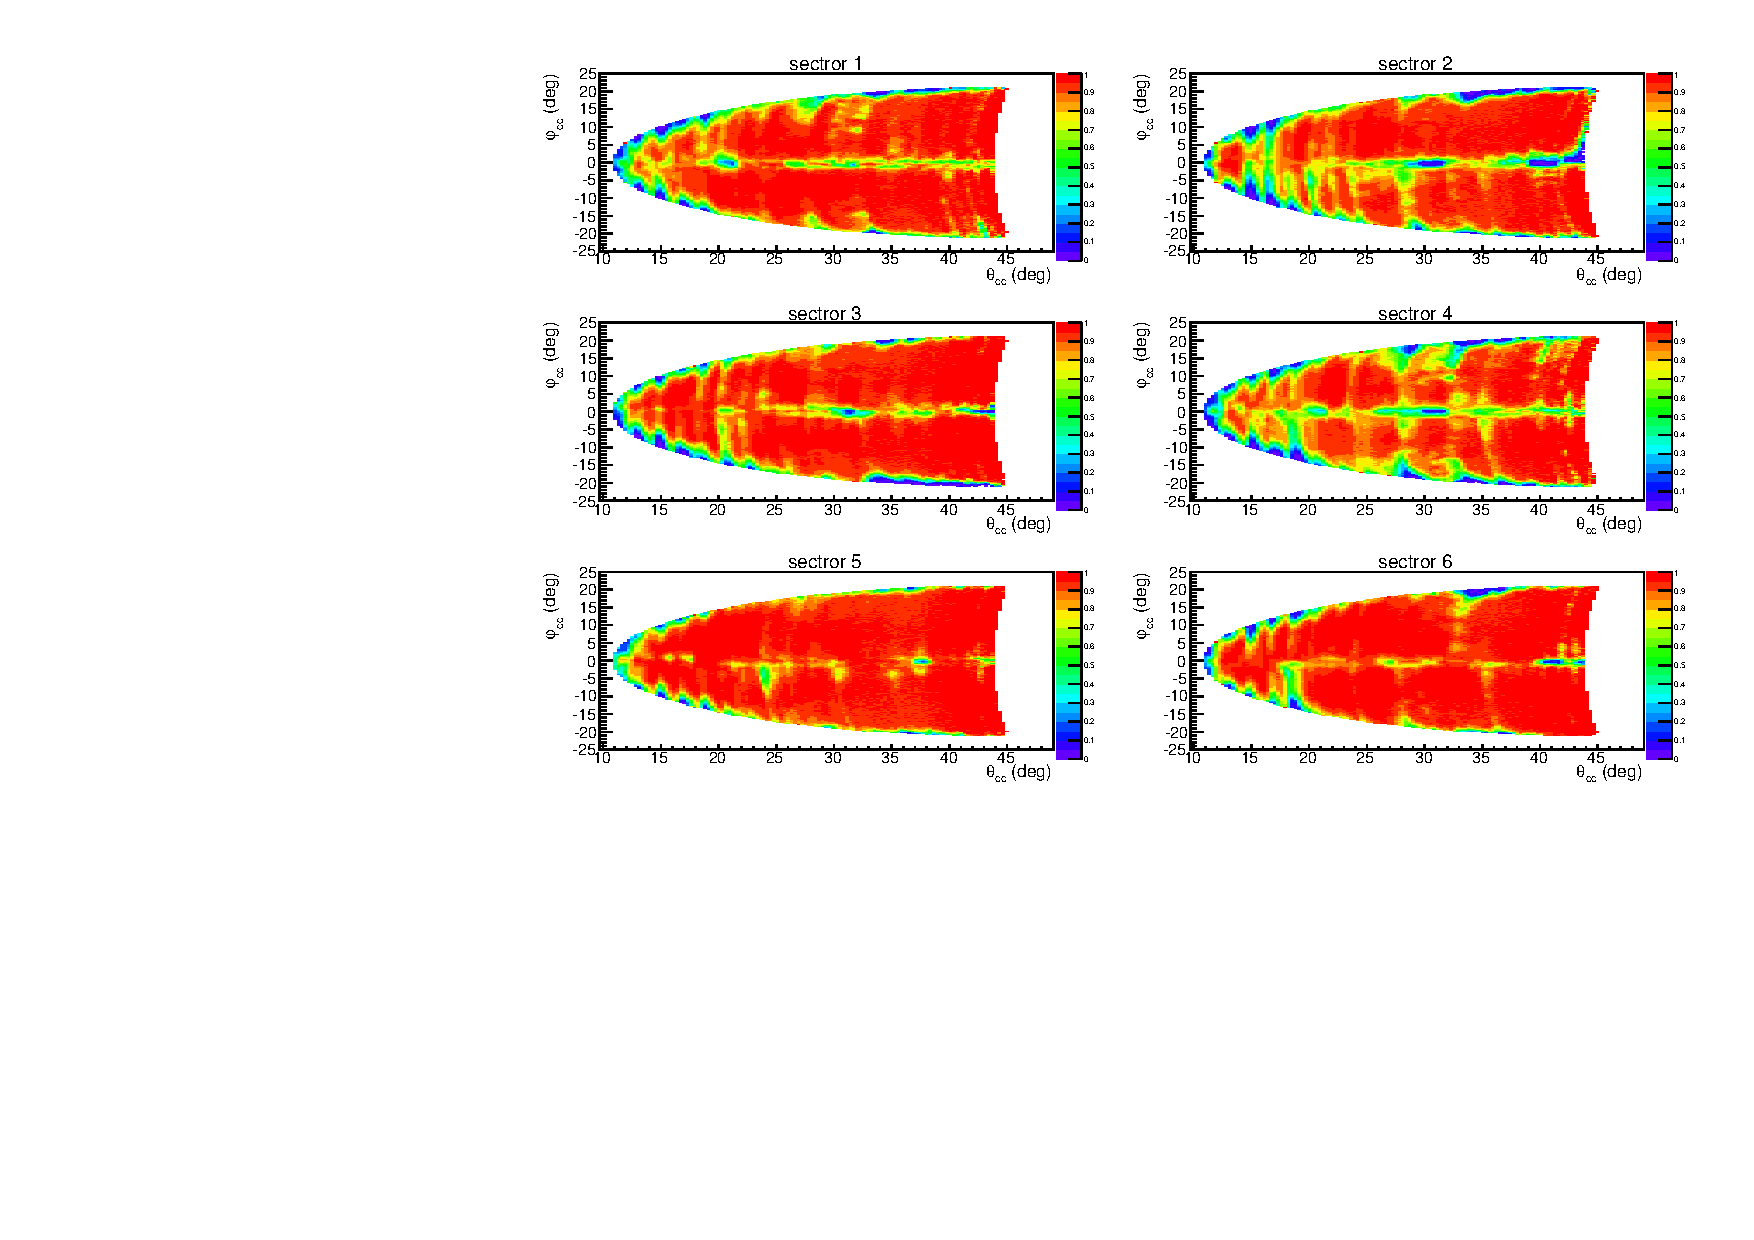
\includegraphics[width=12cm]{pictures/event_selection/cc_cut/ph_vs_th_cc_nocut.pdf}}
\caption{\small  Distributions of the quantity~\ref{eq:cc_ratio} as function of the polar ($\theta_{cc}$) and azimuthal ($\varphi_{cc}$) angles in the CC plane for six CLAS sectors.} \label{fig:ph_vs_th_cc}
\end{center}
\end{figure}

\begin{figure}[htp]
\begin{center}
\framebox{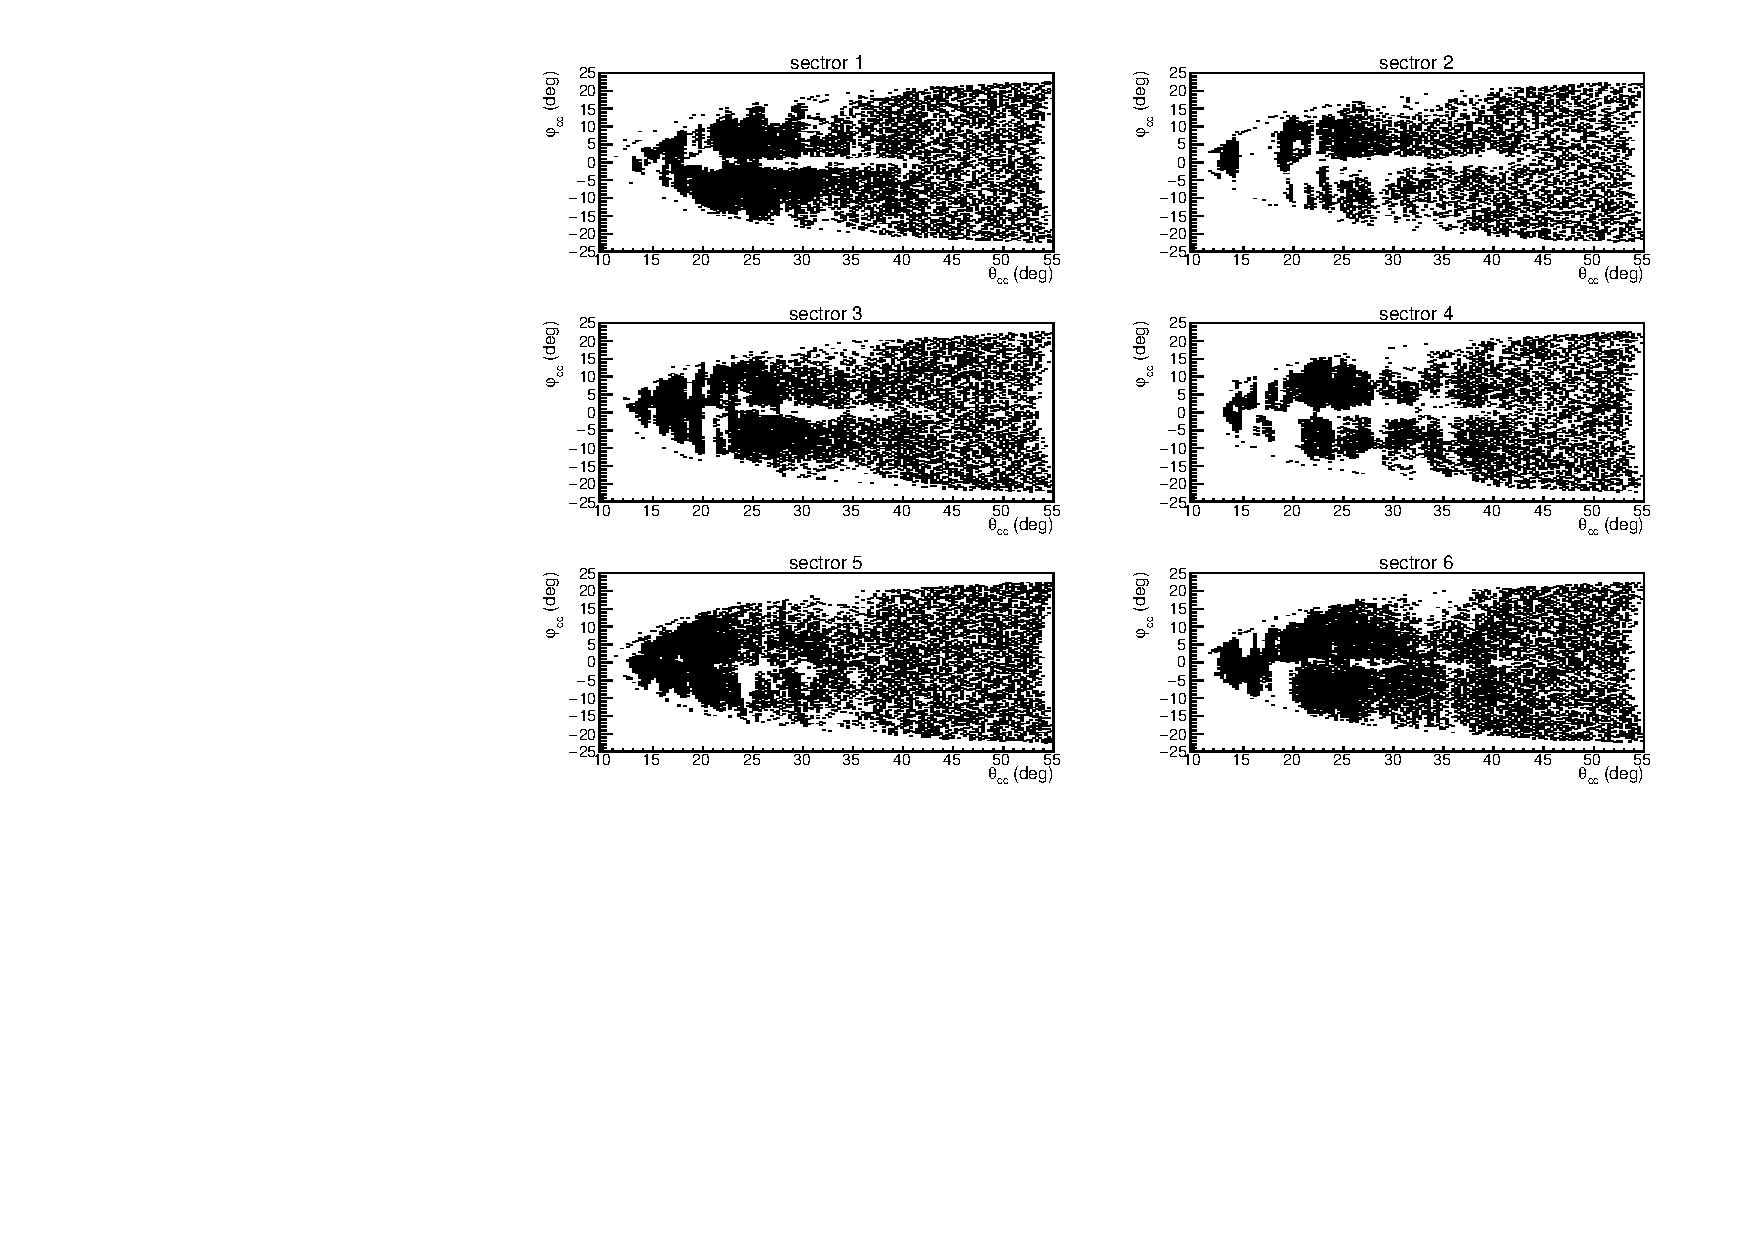
\includegraphics[width=12cm]{pictures/event_selection/cc_cut/ph_vs_th_cc_08cut.pdf}}
\caption{\small  Zones where CC is efficient enough to accept good electron candidates are shown in black as function of the polar ($\theta_{cc}$) and azimuthal ($\varphi_{cc}$) angles in the CC plane for six CLAS sectors. } \label{fig:ph_vs_th_cc_08cut}
\end{center}
\end{figure}

After the geometrical cut shown in Fig.~\ref{fig:ph_vs_th_cc_08cut} is applied photoelectron distributions are plotted for each PMT on the left and right sides of each CC segment and for each CLAS sector (see Fig.~\ref{fig:nphe_cut}). The segment number and $index$ that indicates which side PMT was fired are taken from the  CCPB bank $Status$ variable according to

\begin{equation}
Status = 10\times(\text{CC segment number}) + 1000\times( 1 + index),
\label{eq:cc_segment}
\end{equation}
where $index$ is 1 for right PMTs, -1 for left PMTs, and 0 for the case when both PMTs were fired.

As it is seen in Fig.~\ref{fig:nphe_cut}, there are some peaks at low number of photoelectrons. These peaks correspond to $\pi^{-}$ contamination and/or noise in PMTs~\cite{Osipenko:2004}. To eliminate events under this peak all events on the left side of the red vertical line in Fig.~\ref{fig:nphe_cut} are excluded from the analysis.

Since Monte Carlo does not reproduce photoelectron distributions well enough, the cut shown by the red line in Fig.~\ref{fig:nphe_cut} is applied only to the data. To recover good electrons that were cut off in this way a special procedure is developed. The part of the distributions on the right side of the red line is fit by function~\ref{eq:cc_Poisson}, which is a slightly modified Poisson distribution. 
\begin{equation}
y = P_{1}\left(\frac{P_{3}^{\frac{x}{P_{2}}}}{\Gamma\left(\frac{x}{P_{2}}+1\right)}
\right)e^{-P_{3}}
\label{eq:cc_Poisson}
\end{equation}

The fitting function is then continued into the region on the left side of the red line. In this way the two regions, shown by blue and green in Fig.~\ref{fig:nphe_cut}, are determined. Finally the correction factors are defined by~\ref{eq:cc_corr_fact} and applied as a weight for each event which goes to the particular PMT.
\begin{equation}
F_{ph.\,\, el.} = \frac{\color{green}{green\,\,  area} \color{black}{\,\,+\,\,} \color{blue}{blue\,\,  area}}{\color{green}{green\,\,  area}}
\label{eq:cc_corr_fact}
\end{equation}

It needs to be mentioned that segments one, two, and 18 are removed from the analysis completely since they are dominated by events with very low number of photoelectrons. The procedure described above is applied for left and right side PMTs. For the events with both PMTs fired the peak at low number of photoelectrons is almost absent and no additional cut like this is needed.

%Segment from CCPB bank: segment = (status\%1000)/10. PMT from CCPB: pmt = (status/1000)-1.\\


\begin{figure}[htp]
\begin{center}
\framebox{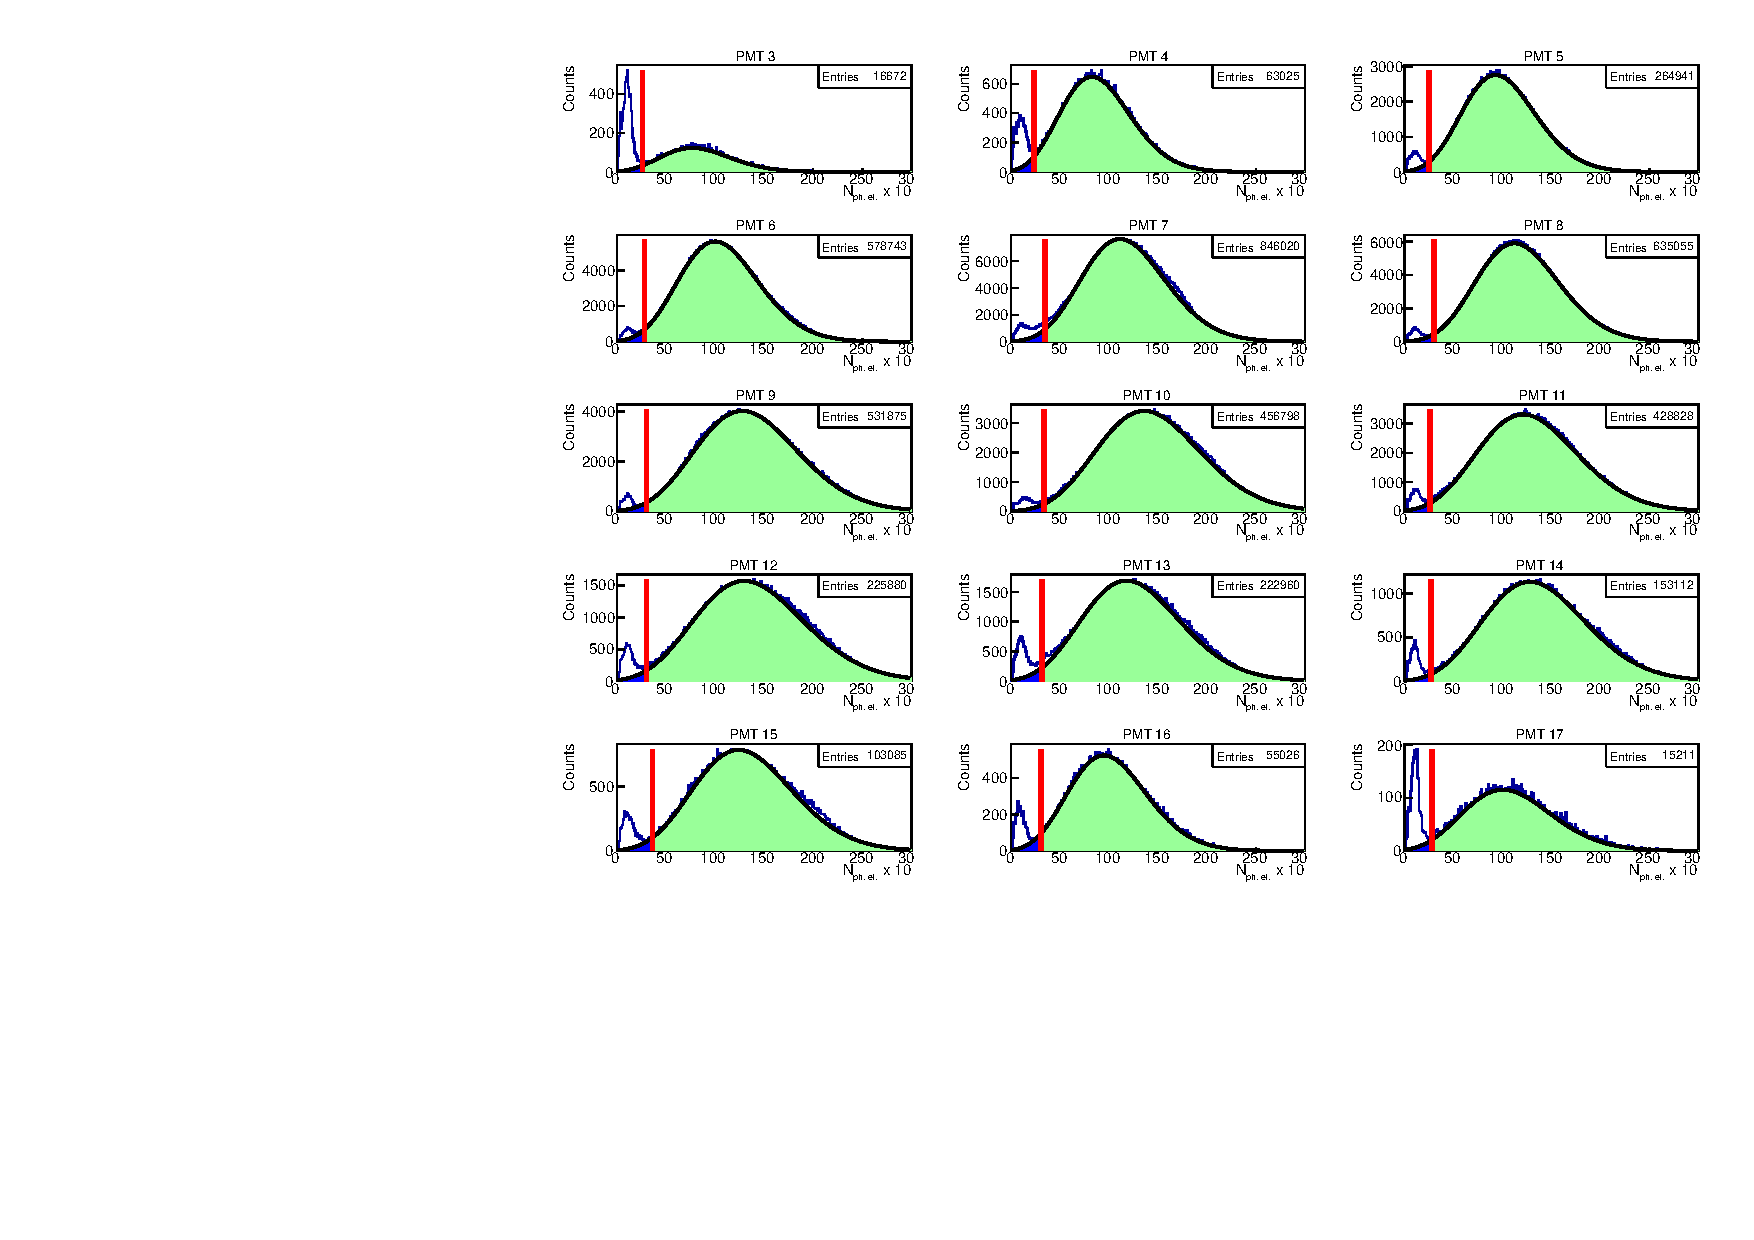
\includegraphics[width=12cm]{pictures/event_selection/cc_cut/nphe_cut.pdf}}
\caption{\small  Number of photoelectrons multiplied by ten for the left side of sector one of CC. Various plots correspond to various CC segments. Black curves show the fit by function~\ref{eq:cc_Poisson}. Red vertical lines show the applied cut. Regions that are needed to calculate the ratio~\ref{eq:cc_corr_fact} are shown in blue and green.} \label{fig:nphe_cut}
\end{center}
\end{figure}





\subsection{Hadron identification}
\label{hadron}

The CLAS time-of-flight (TOF) system provides information on particle
velocity $(\beta= v/c)$.  The information from the Drift
Chambers allows to measure the particle momentum $(P)$. Therefore,
charged hadron can be identified using the relation between particle
mass, momentum, and velocity
\begin{equation}
\beta=\frac{p}{\sqrt{p^{2}+m^{2}}}.
\label{eq:hadron_hadronmass}
\end{equation}

For the hadron identification, only events with electron candidates that have been selected in the previous step are used.
$\beta$ versus momentum distributions are plotted for each TOF scintillator in each CLAS sector (see example plots for CLAS sector one in Fig.~\ref{fig:b_vs_p_positive} for positively charged particles and in Fig.~\ref{fig:b_vs_p_negative} for preliminary selected $\pi^{-}$ candidates). 

It needs to be mentioned that in order to simplify the analysis process the preliminary particle id was made on an initial step of converting data from the BOS files to the files with ROOT trees. It leads to the fact that in 
Figure~\ref{fig:b_vs_p_negative} only the region that corresponds to the preliminary selected $\pi^{-}$ candidates is filled with events.

For visual identification of improperly working scintillation bars, theoretical curves with hadron~\ref{eq:hadron_hadronmass} ($\pi^{+}$, $\pi^{-}$, proton) proper mass assumptions are plotted. As it can be seen in the plots paddle number 48 has enormous number of events. It happened most likely, because more paddles of TOF were connected to TDC 48 or due to cooking problems. Therefore, paddles 48 are excluded from the analysis. Besides scintillators number 17 in sectors two and five worked improperly and are also excluded from the analysis. 

Events between purple dashed curves in Fig.~\ref{fig:b_vs_p_positive} and Fig.~\ref{fig:b_vs_p_negative} are selected as $\pi^{+}$ and $\pi^{-}$ candidates, respectively. Analytical formulae for these curves are given in~\ref{eq:hadron_pioncuts}.
\begin{equation}
\begin{aligned}
\beta <
\frac{(205.98-P_{hadron})\left(\frac{200.-P_{hadron}}{200.+P_{hadron}}\right)^{0.7}(P_{hadron}+0.5)}
{(200.02+P_{hadron})\sqrt{(P_{hadron}+0.5)^{2}+0.019}} + 0.019 \\
\beta > \frac{(1.+5.\times1.07\times(P_{hadron}-0.07))(P_{hadron}-0.07)}
{(1.+5.(P_{hadron}-0.07))\sqrt{(P_{hadron}-0.07)^{2}+0.138^{2}}} - 0.1
\label{eq:hadron_pioncuts}
\end{aligned}
\end{equation}

For proton candidates the selection cuts~\ref{eq:hadron_protoncuts} are used. They are shown by the red dashed lines in Fig.~\ref{fig:b_vs_p_positive}. 
%One the Fig.~\ref{fig:b_vs_p_negative}  events in the area of this cut are not shown because there are negative particles with so high masses in the investigated reaction. So, they are were removed on level of very preliminary $\pi^{-}$ candidates selection.
\begin{equation}
\begin{aligned}
\beta <
\left(\frac{P_{hadron}}{\sqrt{P_{hadron}^{2}+0.938^{2}}}+0.02\right)\frac{1.2+0.92P_{hadron}}{1.+P_{hadron}}
\label{eq:hadron_protoncuts} \\
\beta > \left(\frac{P_{hadron}}{\sqrt{P_{hadron}^{2}+0.938^{2}}}-0.05\right)
\frac{1.+P_{hadron}}{0.9+1.06P_{hadron}} 
\end{aligned}
\end{equation}

As seen in Figs.~\ref{fig:b_vs_p_positive} and \ref{fig:b_vs_p_negative} some scintillators with numbers larger equal 40 have two bands (both of them most likely correspond to 
the given hadron). The origin of these two bands can be based on mistakes in data cooking/calibration or the consequence of the fact that two scintillation bars are connected to one TDC. For this large-number scintillators all events laying higher than the upper cut for protons are assumed to be pions.

%only one cut~\ref{eq:hadron_high_paddles} shown by dashed orange curves on Figs.~\ref{fig:b_vs_p_positive},\ref{fig:b_vs_p_negative} was applied. All events laying higher than that cut assumed as pions candidates. Events below this cut in Fig.~\ref{fig:b_vs_p_positive} assumed as protons.
%\begin{equation}
%\beta <
%\left(\frac{P_{hadron}}{\sqrt{P_{hadron}^{2}+0.938^{2}}}+0.03\right)\frac{1.2+0.92P_{hadron}}{1.+P_{hadron}}
%\label{eq:hadron_high_paddles}
%\end{equation}


\begin{figure}[htp]
\begin{center}
\framebox{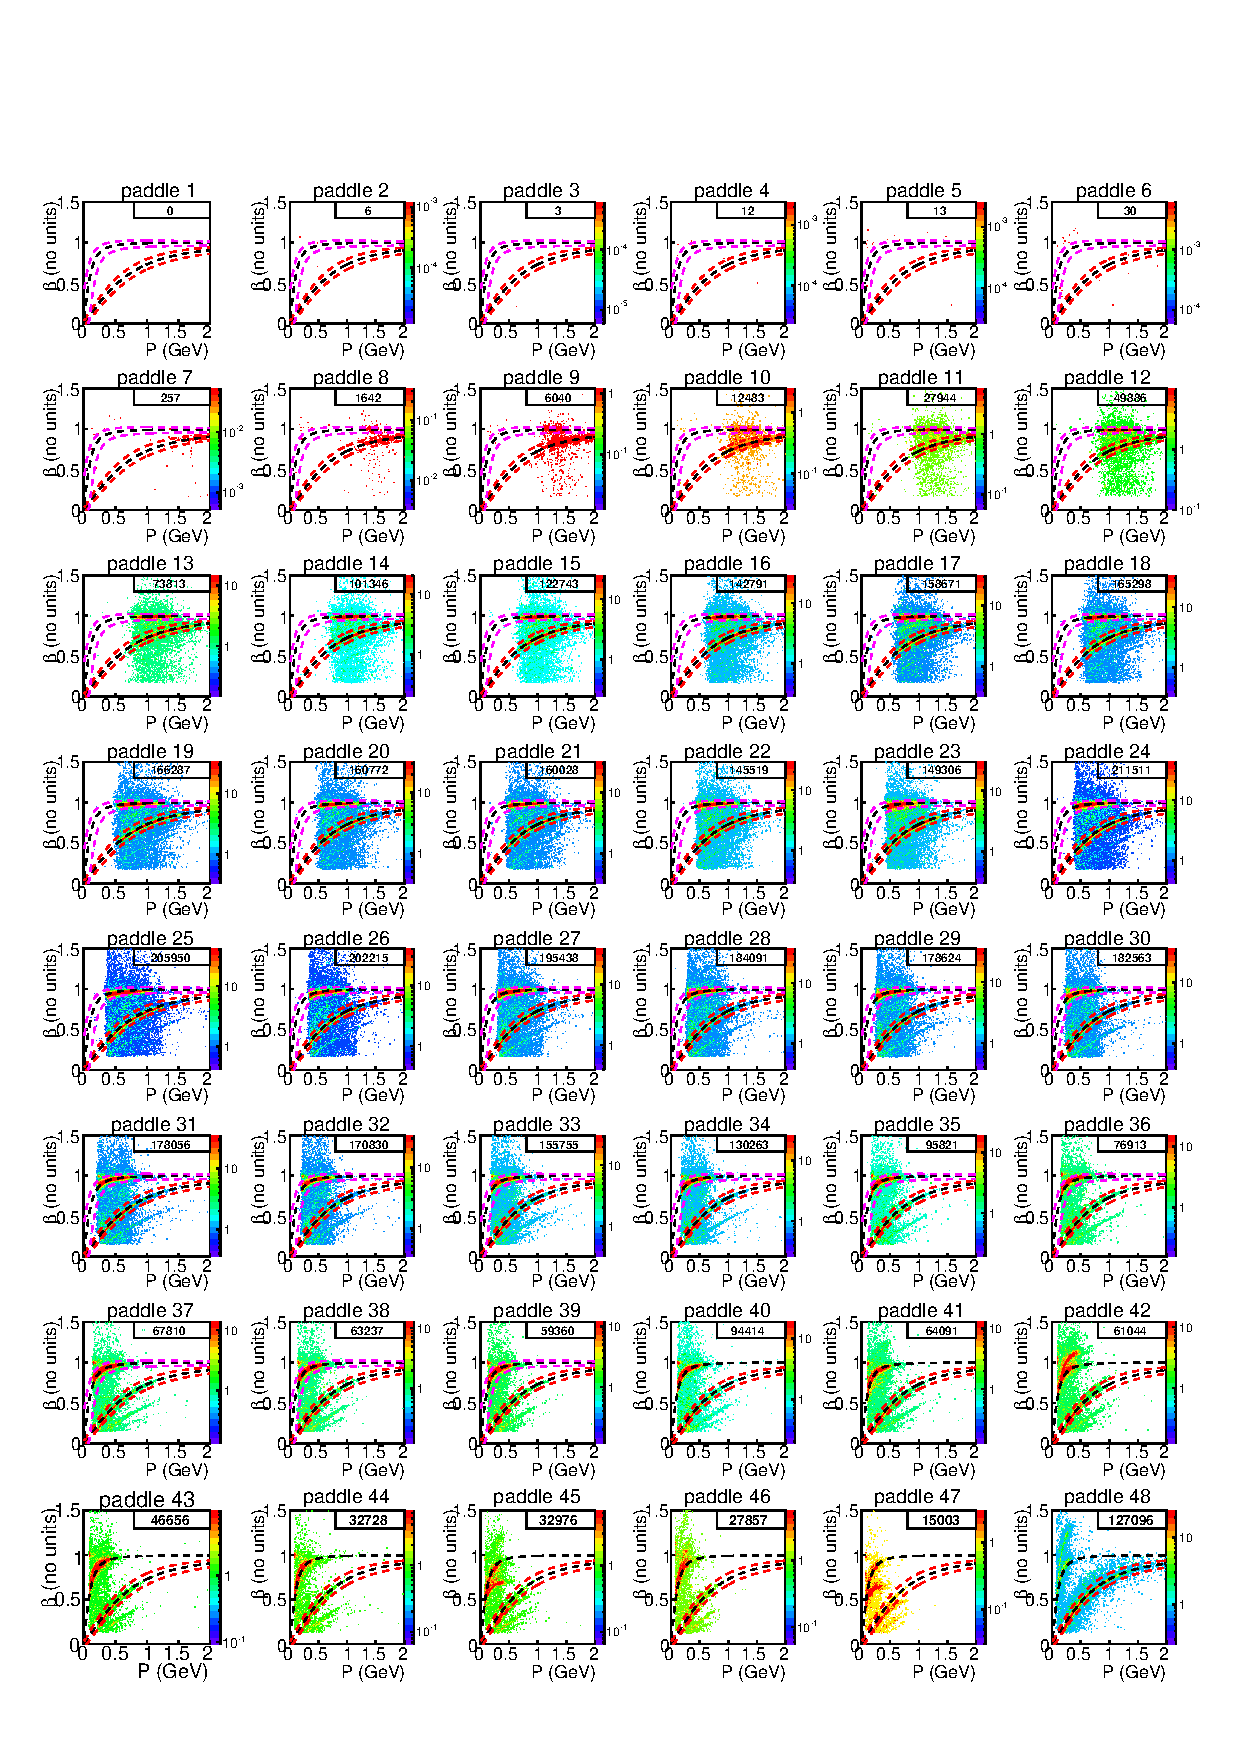
\includegraphics[width=14.5cm]{pictures/event_selection/b_vs_p/b_vs_p_positiv.pdf}}
\caption{\small  $\beta$ versus momentum distributions for positively charged particles for different TOF scintillators in CLAS sector one. Black dashed curves are theoretical under the exact hadron mass assumption~\ref{eq:hadron_hadronmass}. Events between the two purple dashed~\ref{eq:hadron_pioncuts} and two red dashed~\ref{eq:hadron_protoncuts} curves are selected as $\pi^{+}$ and proton candidates, respectively. For scintillators with number greater equal 40 all events laying higher than the upper red dashed curve are assumed as $\pi^{+}$ candidates. Number of events is shown in the right upper corner of each plot. \label{fig:b_vs_p_positive}} 
\end{center}
\end{figure}




\begin{figure}[htp]
\begin{center}
\framebox{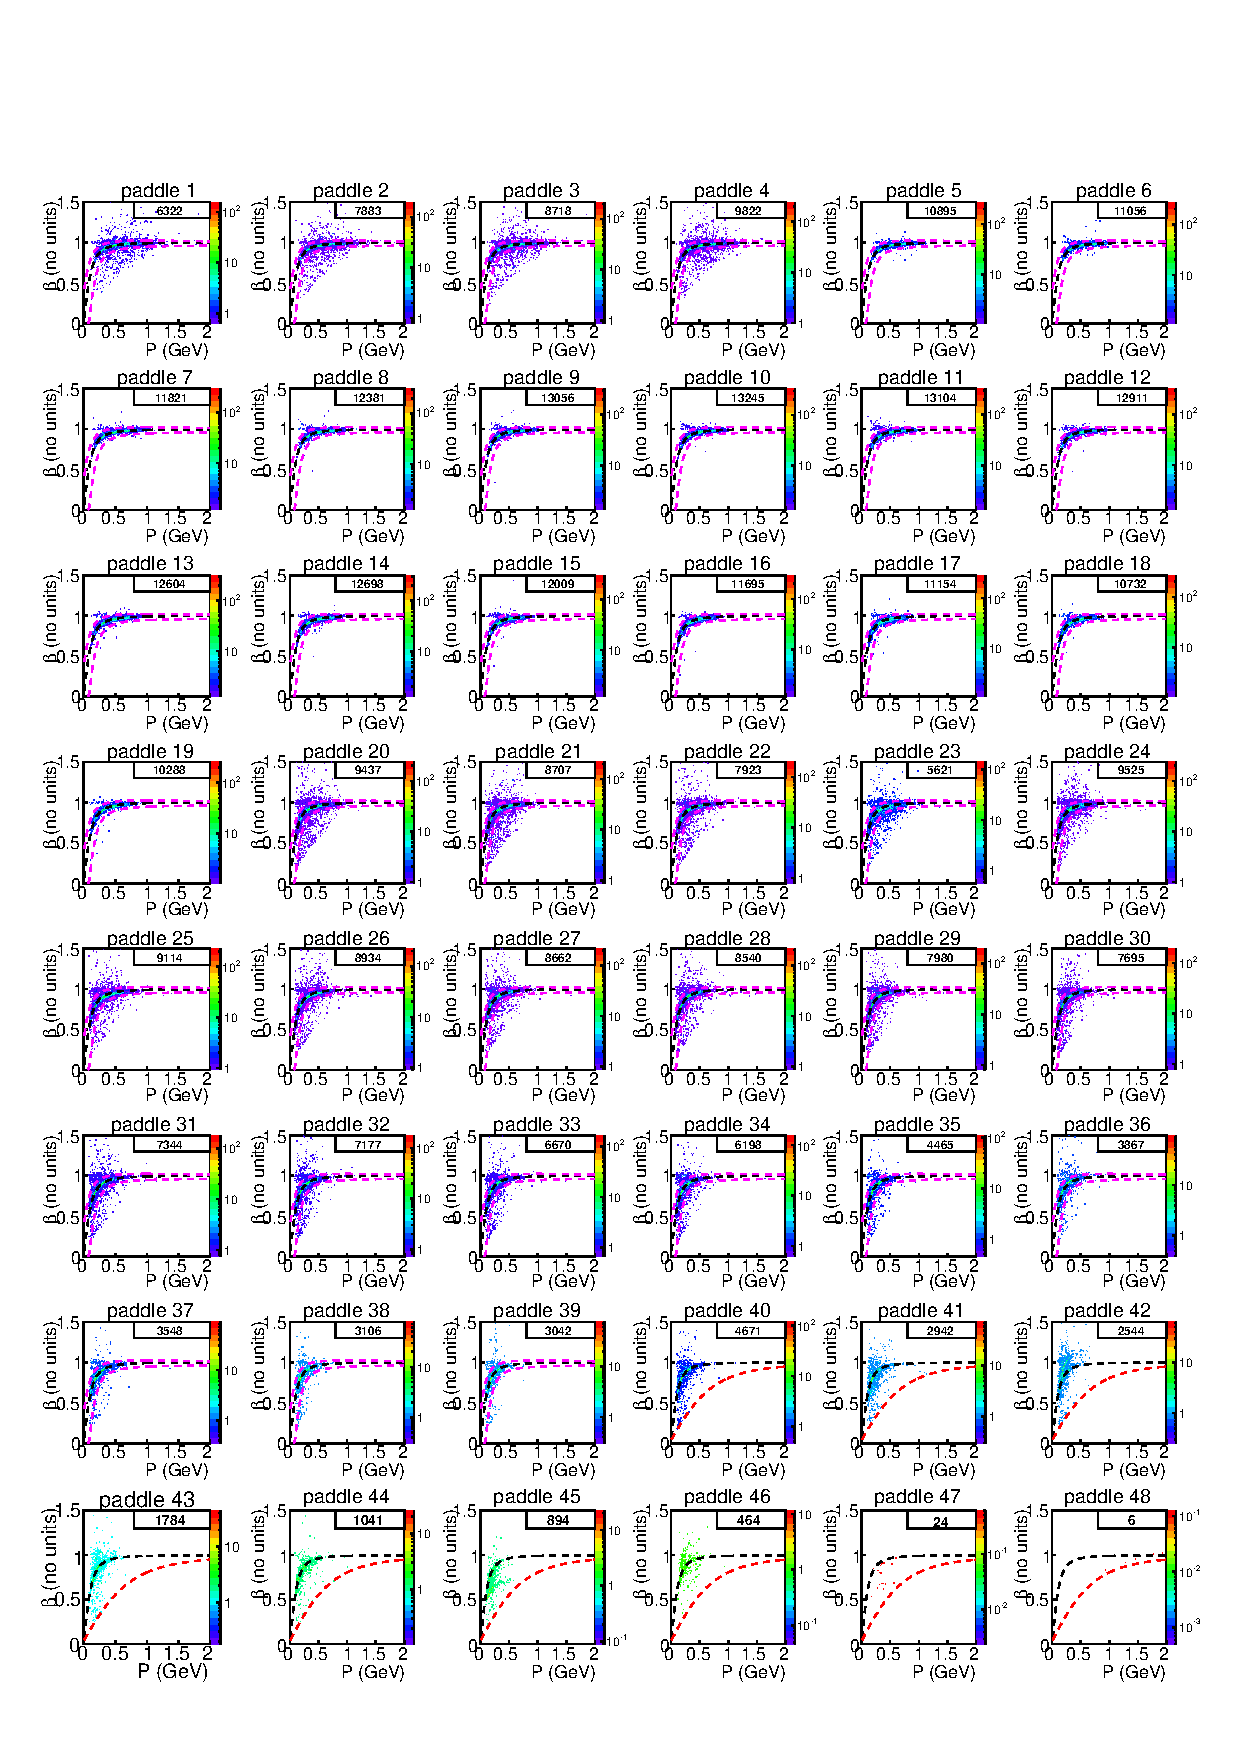
\includegraphics[width=14.5cm]{pictures/event_selection/b_vs_p/b_vs_p_negative.pdf}}
\caption{\small  $\beta$ versus momentum distributions for negatively charged particles for different TOF scintillators in CLAS sector one. Black dashed curves are theoretical under the exact $\pi^{-}$ mass assumption~\ref{eq:hadron_hadronmass}. Events between the two purple dashed~\ref{eq:hadron_pioncuts} curves are selected as $\pi^{-}$ candidates. For scintillators with number greater equal 40 all events laying higher than  the red dashed curve are assumed as  $\pi^{-}$ candidates. Number of events is shown in the right upper corner of each plot. \label{fig:b_vs_p_negative}} 
\end{center}
\end{figure}

\subsection{Timing correction}
\label{time_corr}

Another approach can be used to treat the scintillators with numbers larger equal 40, which have two bands that  correspond to the same hadron. 
The idea of this approach is to plot the difference between the measured time that hadron travels between the target and the SC plane and the same quantity calculated under the exact hadron mass assumption.
This time difference $\Delta T$ is calculated as:

\begin{equation}
\Delta T=\frac{l_{h}}{c}\left ( \frac{1}{\beta_{n} } -\frac{1}{\beta _{old}}\right ),
\label{eq:time_corr_delta_T}
\end{equation}
where $l_{h}$ is the hadron path length from the vertex to the SC plane (the $Path$ variable in DCPB bank), $\beta_{n}$ is the nominal $\beta$ with the exact mass of the hadron assumed (see Eq.~\ref{eq:hadron_hadronmass}), $\beta_{old}$ is the value of $\beta$ that needs to be corrected, $c$ is the speed of light.

In the left side in Fig.~\ref{fig:time_corr} $\Delta T$ is plotted for the $\pi^{+}$ candidates for the paddle 42 in CLAS sector one as a function of their momentum. The two horisontal bands are clearly seen in this figure. One of them is around $\Delta T = 0$, while another one is shifted by two nano seconds and corresponds to the wrong band in $\beta$ versus momentum distribution for paddle 42 (see Fig.~\ref{fig:b_vs_p_positive}).




\begin{figure}[htp]
\begin{center}
\framebox{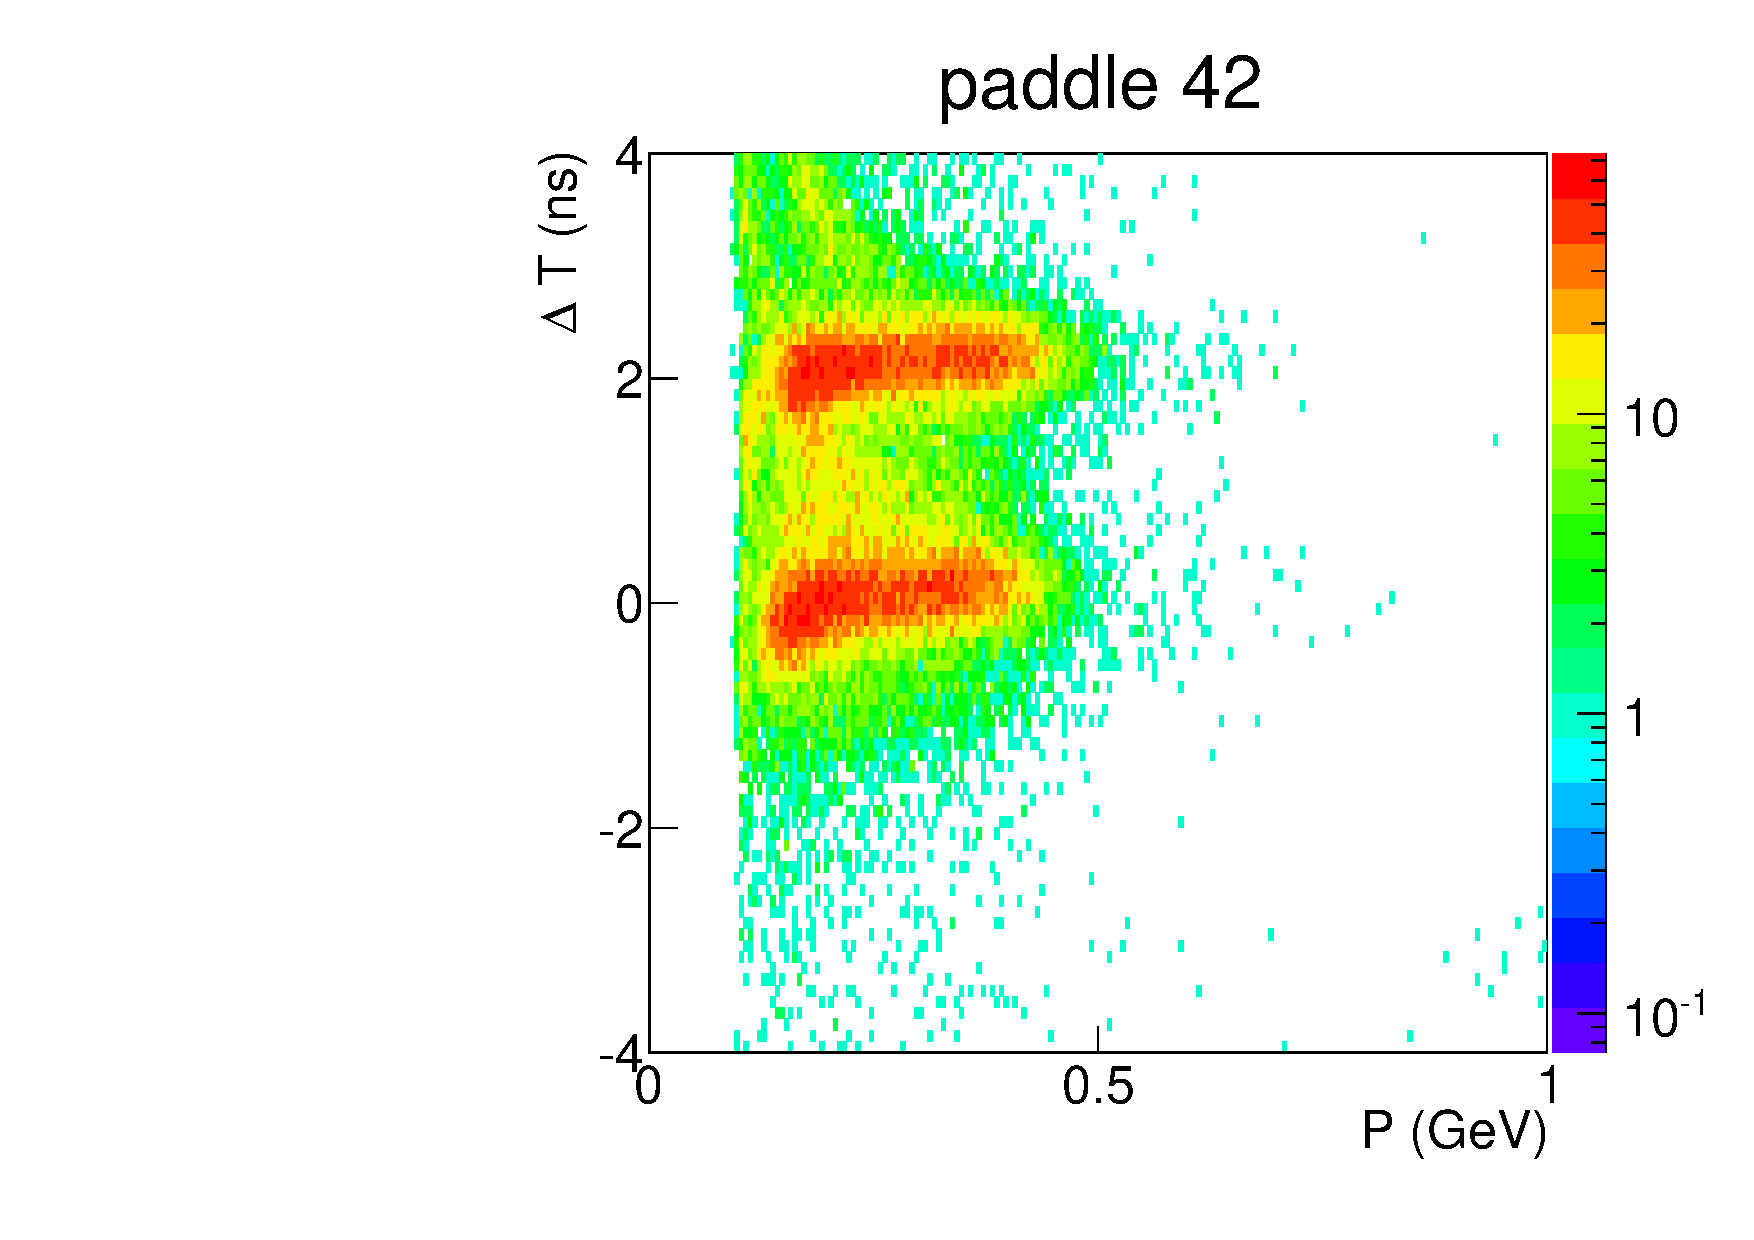
\includegraphics[width=7cm]{pictures/event_selection/b_vs_p/delta_t.pdf}}
\framebox{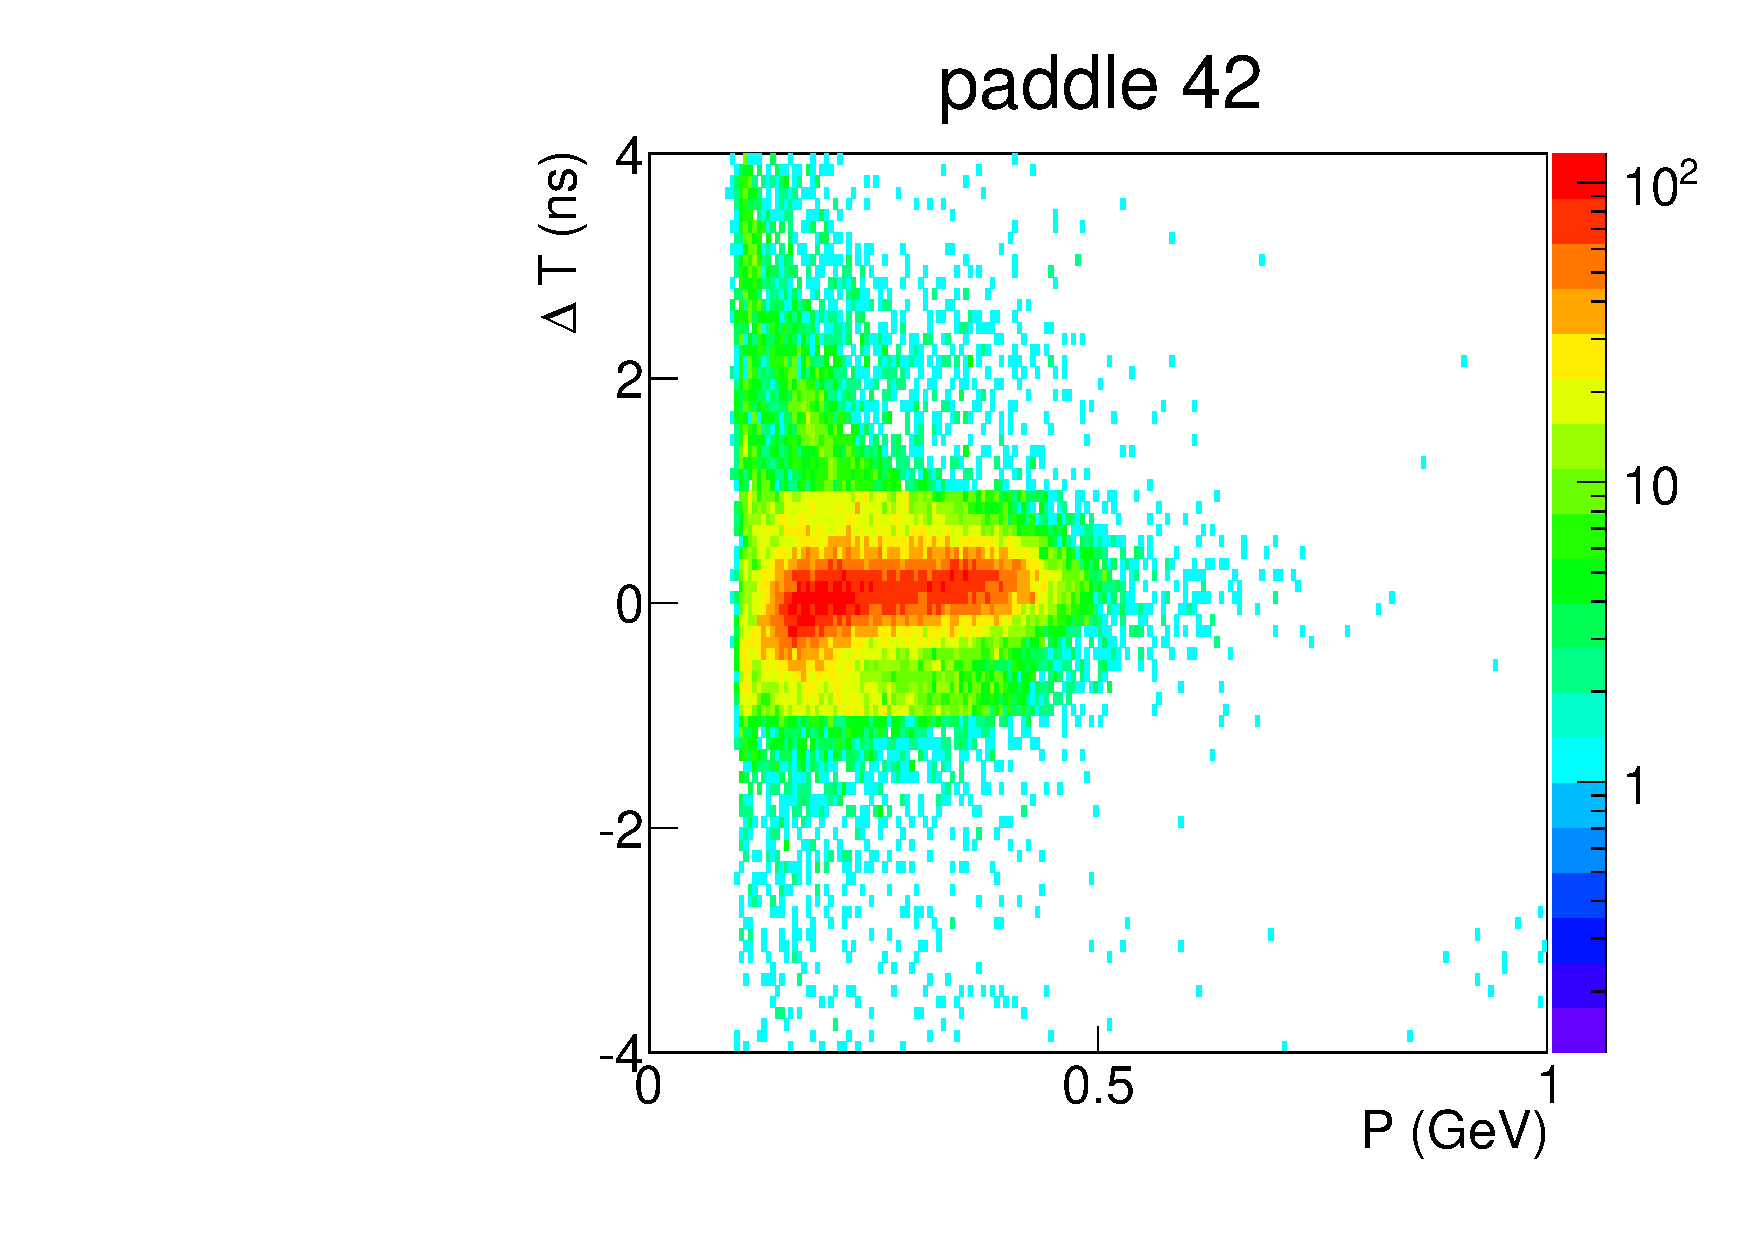
\includegraphics[width=7cm]{pictures/event_selection/b_vs_p/delta_t_time_corr.pdf}}
\caption{\small  Quantity $\Delta T$ that is given by Eq.~\ref{eq:time_corr_delta_T} before (left plot) and after (right plot) the timing corrections. \label{fig:time_corr}} 
\end{center}
\end{figure}

The idea of timing corrections is to shift the wrong bands in $\Delta T$ versus momentum distributions to their correct position around $\Delta T = 0$. The result of this shift is shown in the right side in Fig.~\ref{fig:time_corr}. After this shift the correct value of  $\beta$ is calculated using Eq.~\ref{eq:time_corr_beta_corr}.

\begin{equation}
\beta _{corr} = \frac{1}{\frac{1}{\beta _{n}}-\frac{(\Delta T-t_{max})c}{l_{h}}},
\label{eq:time_corr_beta_corr}
\end{equation}
where $t_{max}$ is the position of each wrong band, 2 ns in the example shown in Fig.~\ref{fig:time_corr}.

After applying the procedure that is described above for all pion candidates in all problematic paddles with double bands, the $\beta$ versus momentum distributions are plotted, see Fig.~\ref{fig:b_vs_p_time_corr}. 
As it is seen in Fig.~\ref{fig:b_vs_p_time_corr} there are no paddles with double bands anymore. So, even for scintillators with the numbers greater equal 40 the same $\beta$ versus momentum cuts (see Eq.~\ref{eq:hadron_pioncuts}) can be applied. This procedure is performed for pion candidates only, since the effect of the band doubling in the $\beta$ versus momentum distributions  for the protons is rather small and all proton candidates are lying inside the cut given by Eq.~\ref{eq:hadron_protoncuts} even without timing corrections.

\begin{figure}[htp]
\begin{center}
\framebox{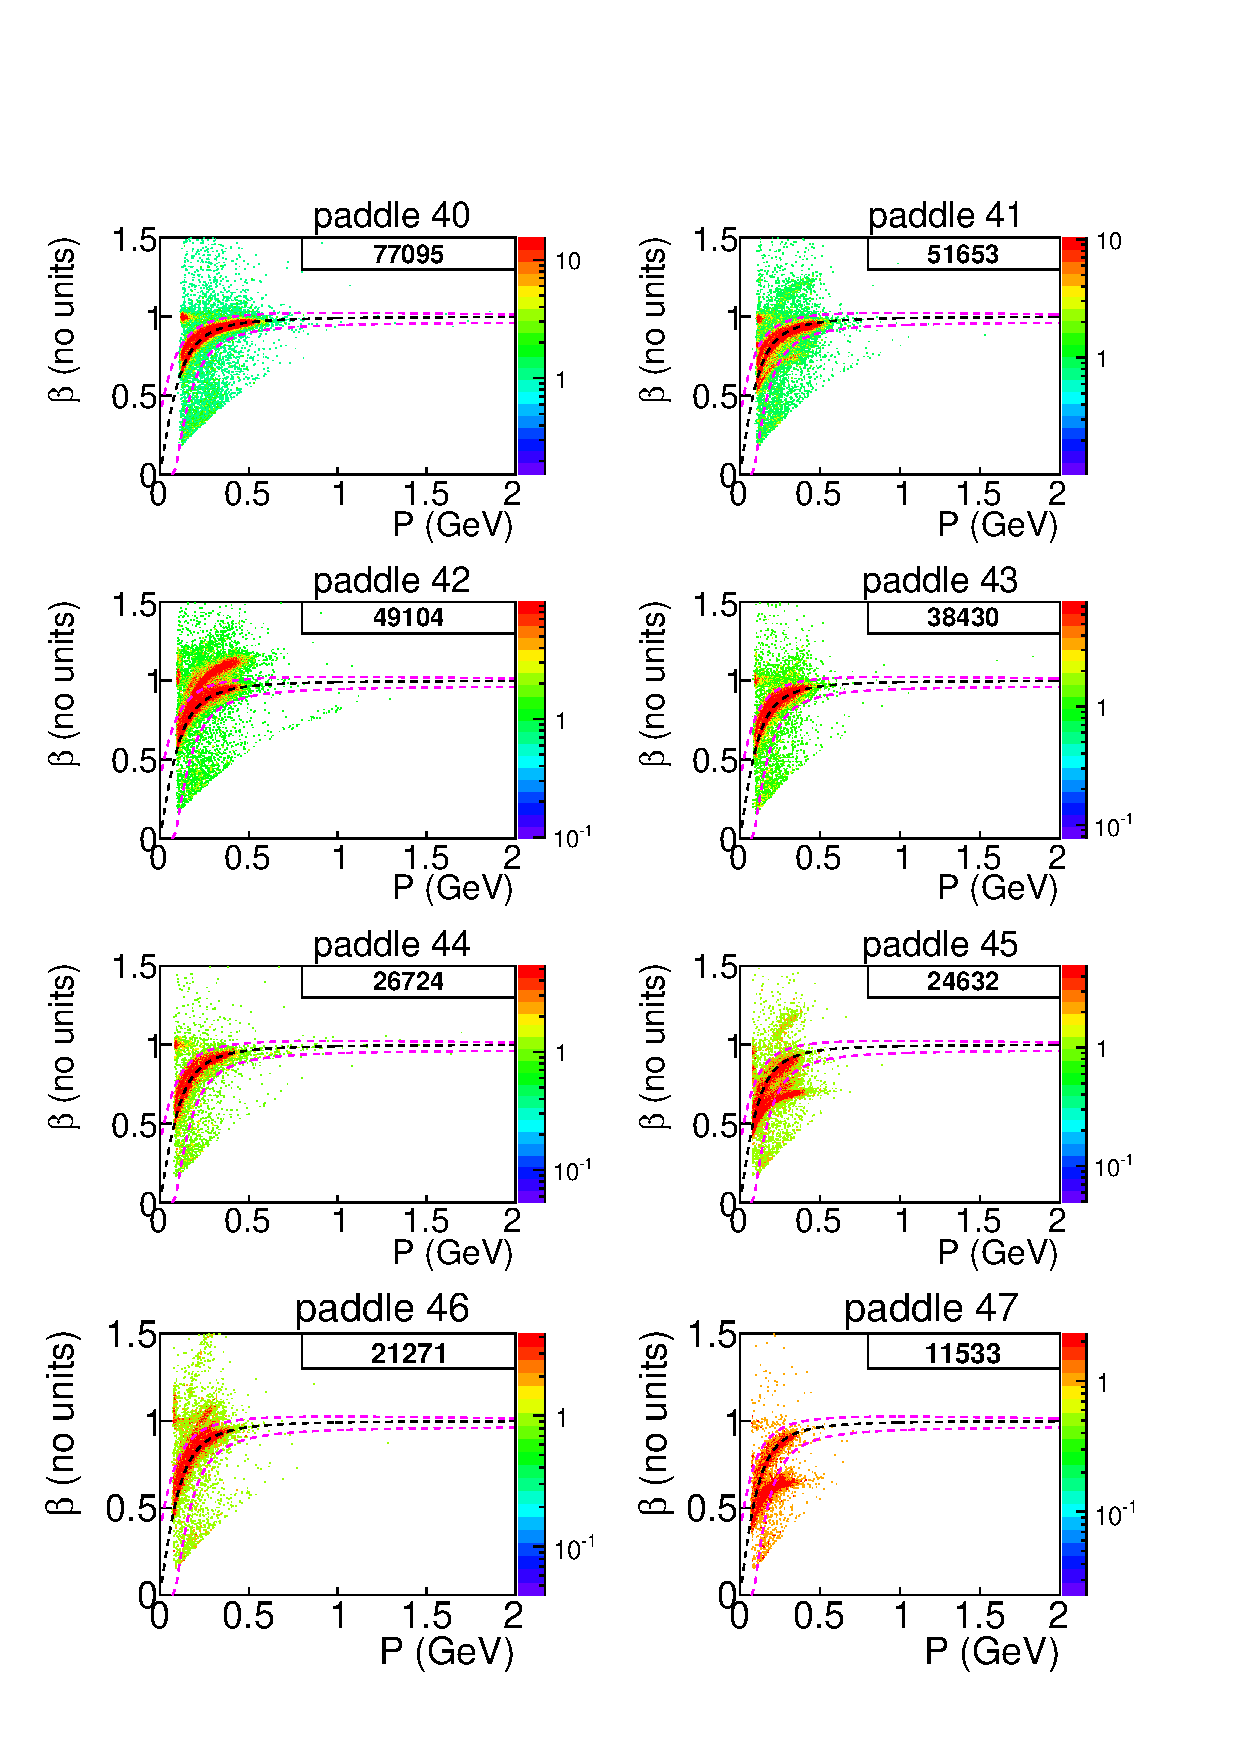
\includegraphics[width=7.5cm]{pictures/event_selection/b_vs_p/b_vs_p_positiv_no_time_corr_new.pdf}}
\framebox{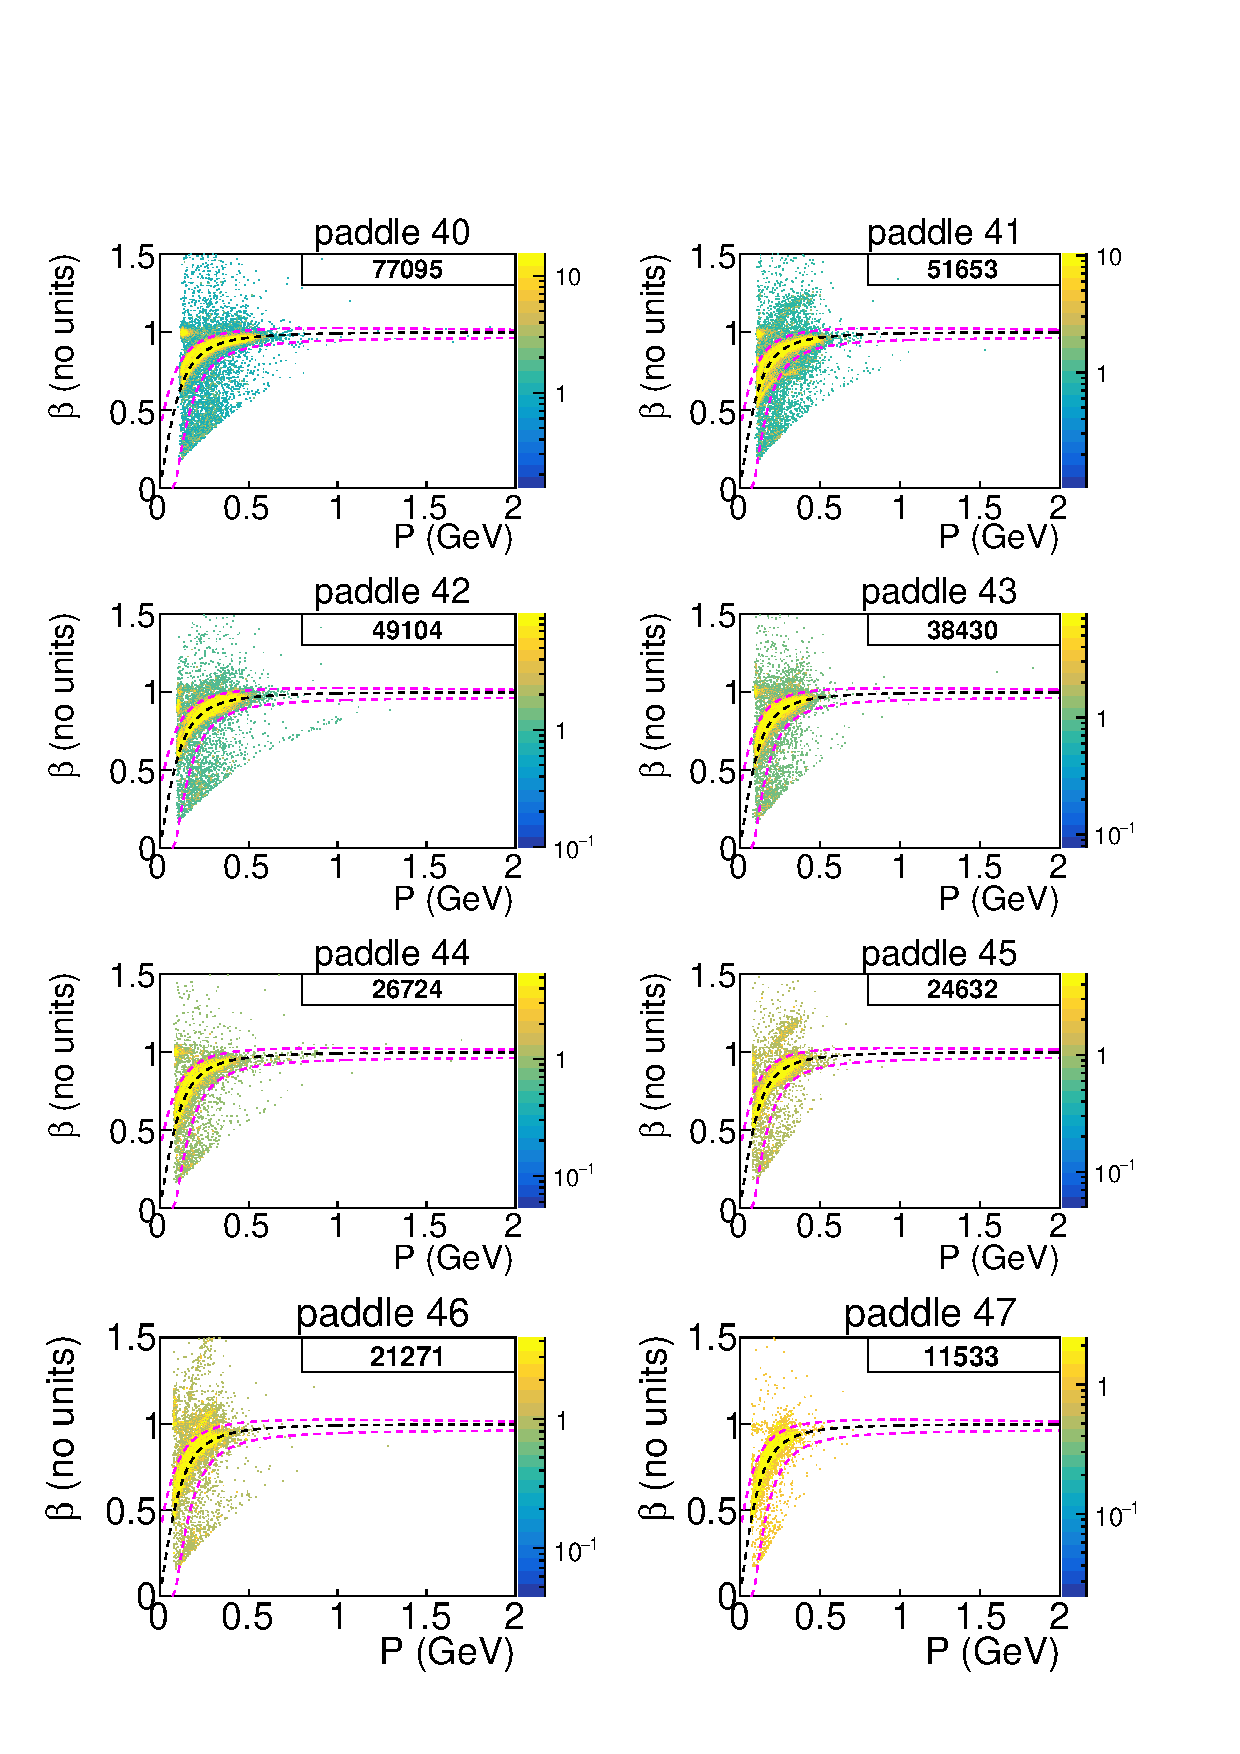
\includegraphics[width=7.5cm]{pictures/event_selection/b_vs_p/b_vs_p_positiv_time_corr_new.pdf}}
\caption{\small  $\beta$ versus momentum distributions before (left plot) and after (right plot) the timing corrections for $\pi^{+}$. Only scintillators in CLAS sector one with number larger than 40 are shown. Black dashed curves are theoretical under the exact $\pi^{+}$ mass assumption~\ref{eq:hadron_hadronmass}. Events between the two purple dashed~\ref{eq:hadron_pioncuts} and two red dashed~\ref{eq:hadron_protoncuts} curves are selected as pions. Number of events is shown in the right upper corner of each plot. \label{fig:b_vs_p_time_corr}} 
\end{center}
\end{figure}

Both methods of hadrons identification that are described in the previous and this sections have been compared and it is found that they give pretty small diference in the cross sections.
Nevertheless, the final cross sections presented in this analysis are obtained using the timing corrections described in this section. 

\section{Momentum corrections}
\label{momcorr}



\subsection{Electron momentum correction}
\label{electronmomcor}

Due to the slight misalignments in the DC position,  small inaccuracies in
the description of the torus magnetic field, and other possible reasons the momentum and angle of
particles may have some small systematic deviations from the real values. 
Since the effects are of unknown origin, they cannot be simulated in GSIM. 
Hence a special momentum correction procedure is needed for the data. The approach~\cite{KPark:momcorr}, which is based on elastic kinematic, was chosen for this purpose. 

Low beam energy $\sim$ 2 GeV of analyzed dataset leads to the small shift ($\sim$ 3 MeV) in elastic peak position. For comparison for 6 GeV runs this shift is about 20 MeV.  
From~\cite{KPark:momcorr} it is known that momentum corrections are essential only for high-energetic particles. Since in $2\pi$ kinematics hadrons carry only small portion of the system momentum,  the expected momentum  corrections for them are significantly less than for electrons and can be neglected.


In Fig.~\ref{fig:el_mom_corr_elast} elastic peak positions are shown for six CLAS sectors before (left panel) and after (right panel) electron momentum correction. The peaks are fit by Gaussians with polynomial background, fitting curves are shown in Fig.~\ref{fig:el_mom_corr_elast}, and the fit parameter $p1$ corresponds to the elastic peak position.  As seen in Fig.~\ref{fig:el_mom_corr_peak_position}, elastic peak positions for all CLAS sectors get closer to the proton mass, shown by red horizontal line. The momentum resolution for electrons can be roughly estimated from  elastic peak width that is about nine MeV.
\begin{figure}[htp]
\begin{center}
\framebox{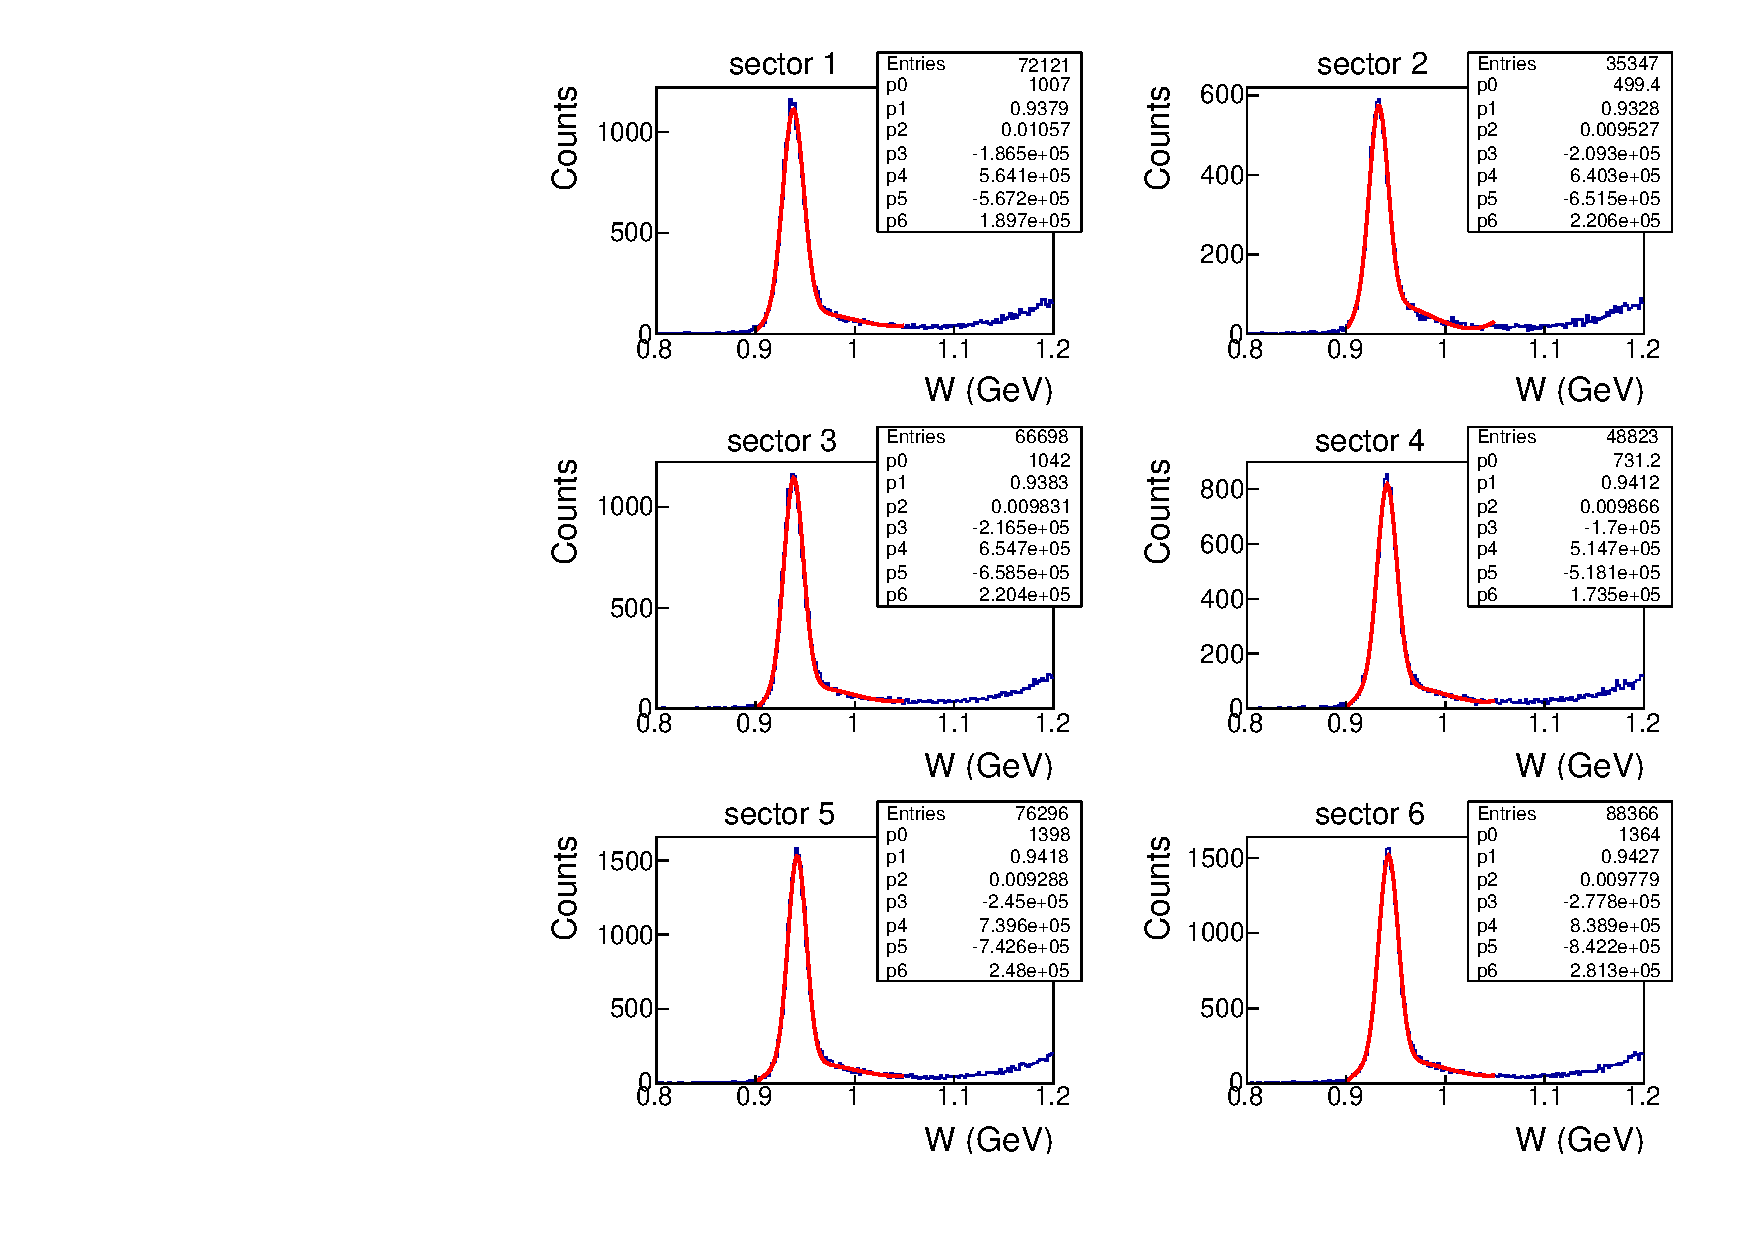
\includegraphics[width=7cm]{pictures/event_selection/mom_corr/elast_before_corr.pdf}}
\framebox{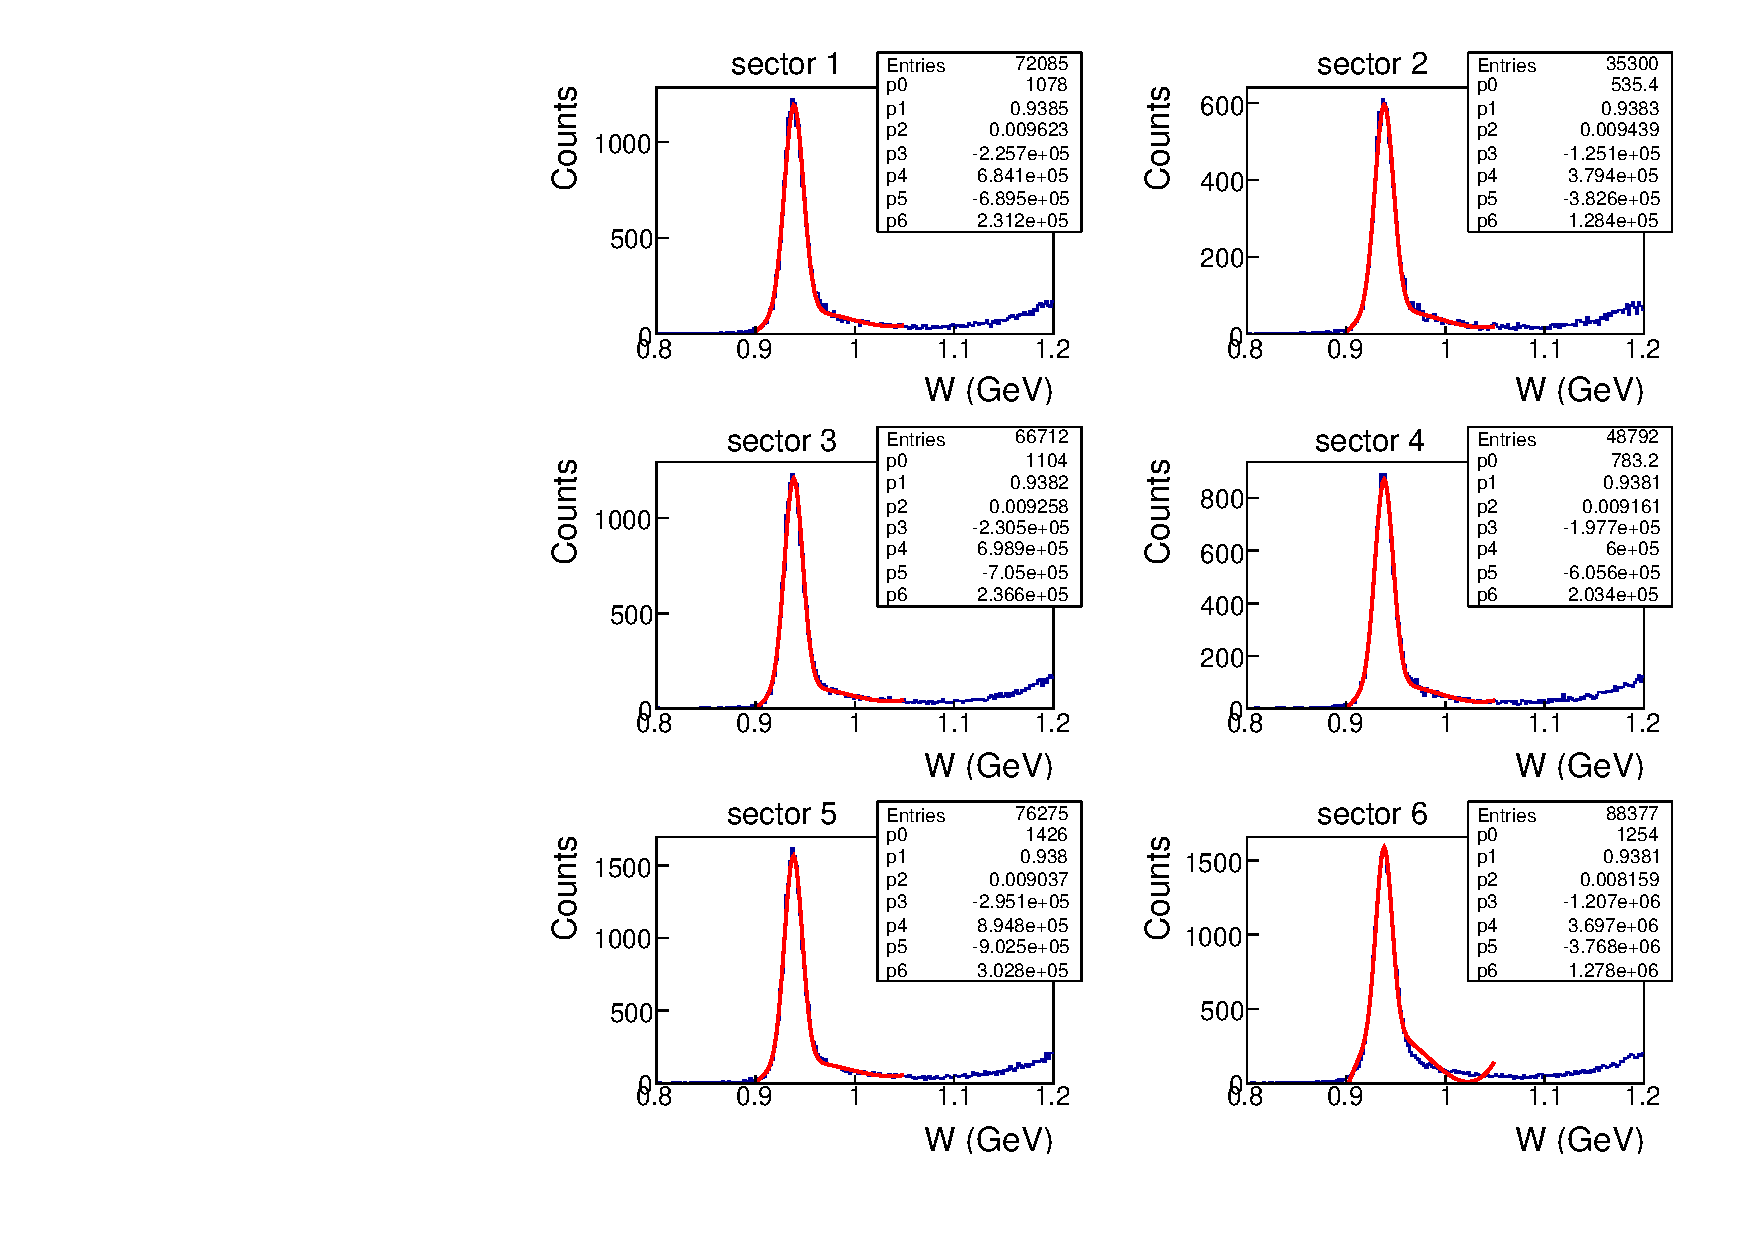
\includegraphics[width=7cm]{pictures/event_selection/mom_corr/elast_after_corr.pdf}
}
\caption{\small Elastic peaks for six CLAS sectors before (left panel) and after (right panel) electron momentum correction. Fit parameter $p1$ corresponds to elastic peak position. \label{fig:el_mom_corr_elast}} 
\end{center}
\end{figure}

\begin{figure}[htp]
\begin{center}
\framebox{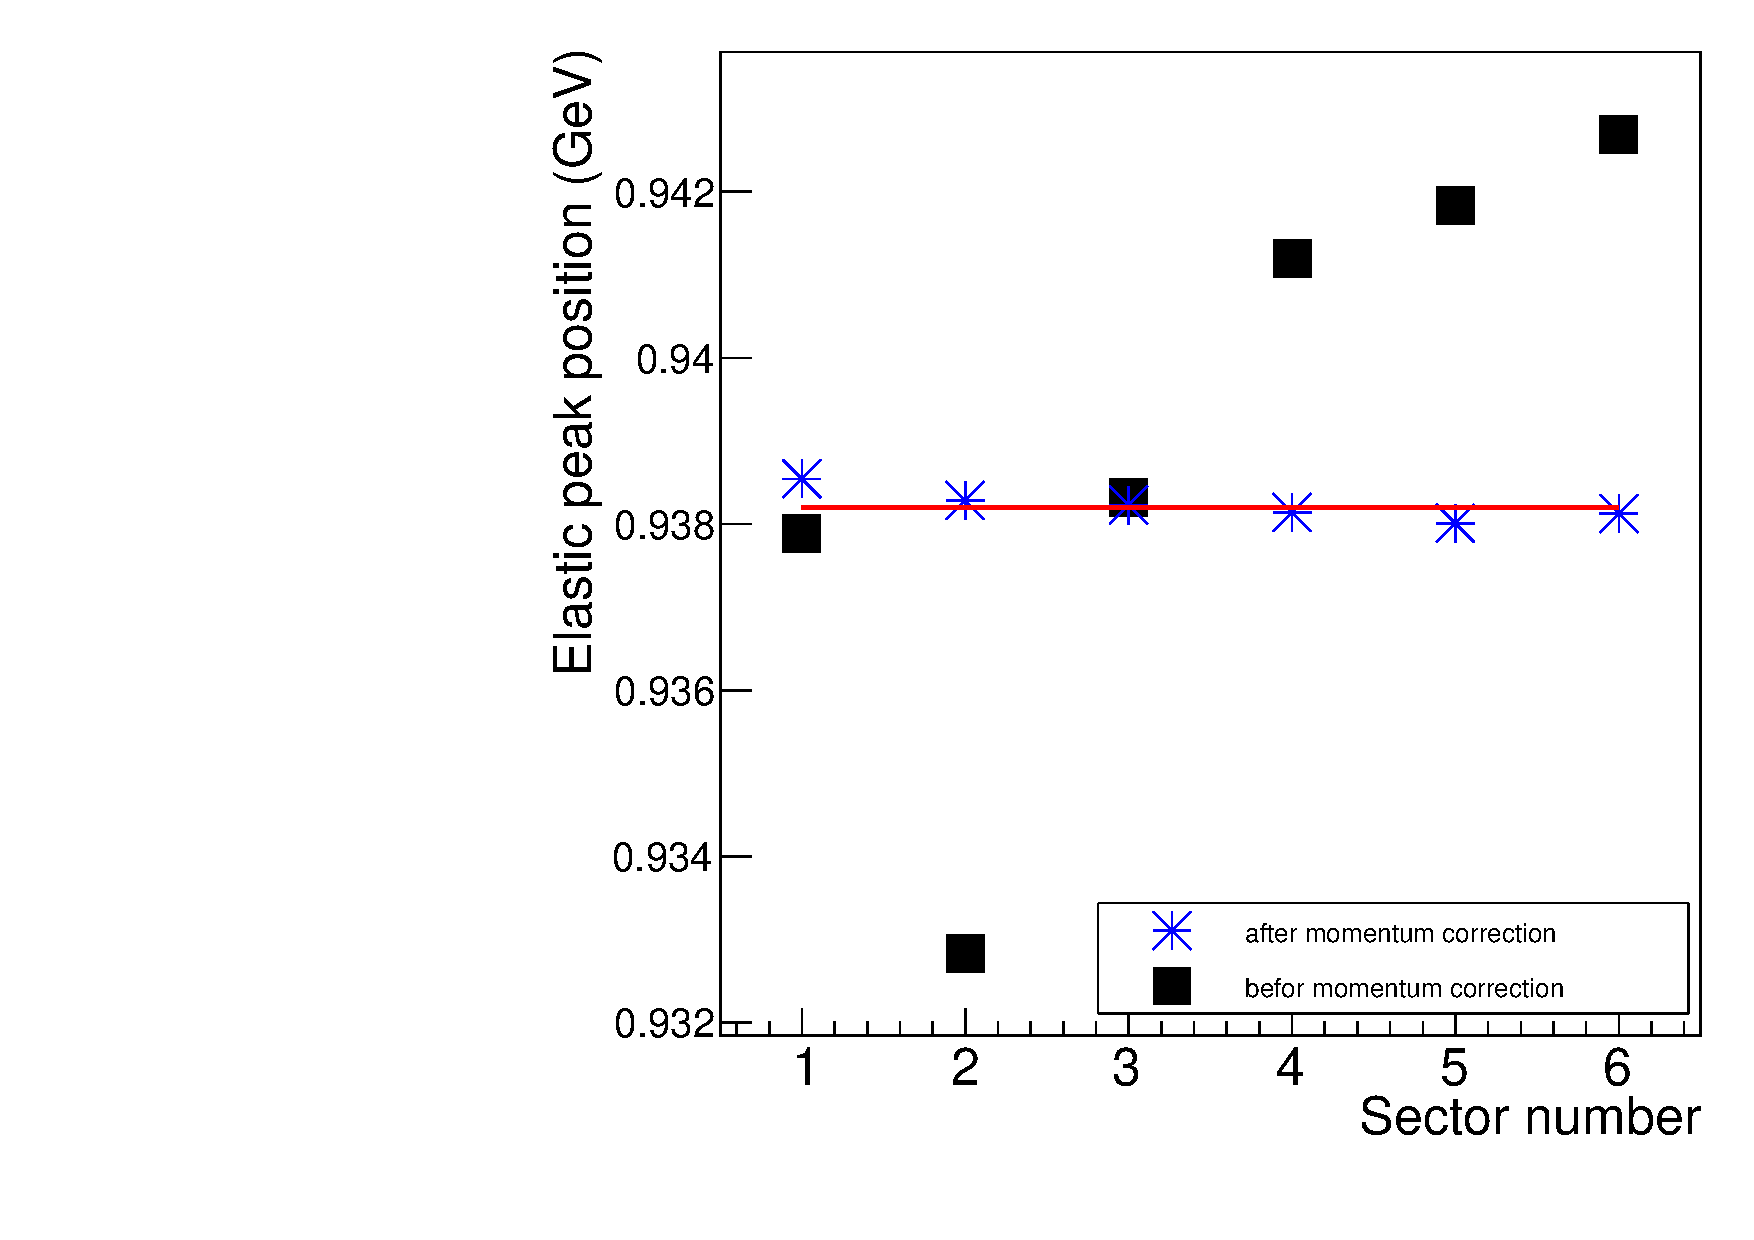
\includegraphics[width=7cm]{pictures/event_selection/mom_corr/elast_pic_position.pdf}}
\caption{\small Elastic peak position for six CLAS sectors before (black squares) and after (blue stars) electron momentum correction. Horizontal red line shows the proton mass. \label{fig:el_mom_corr_peak_position}} 
\end{center}
\end{figure}

Due to unknown reasons (most likely because electrons lose energy when they travel through the detector and target media) the reconstructed electron momentum appears to be slightly lower than the generated one. Therefore, an adapted electron momentum correction procedure is also applied to the Monte Carlo events. This correction depends only on scattered electron angle $\theta$ and momentum, but not on the CLAS sector.   
Figure~\ref{fig:el_mom_corr_sim} shows differences between thrown and reconstructed electron momenta before and after the correction procedure. As shown in Fig.~\ref{fig:el_mom_corr_sim}, these differences become negligible after momentum corrections have been applied.

\begin{figure}[htp]
\begin{center}
\framebox{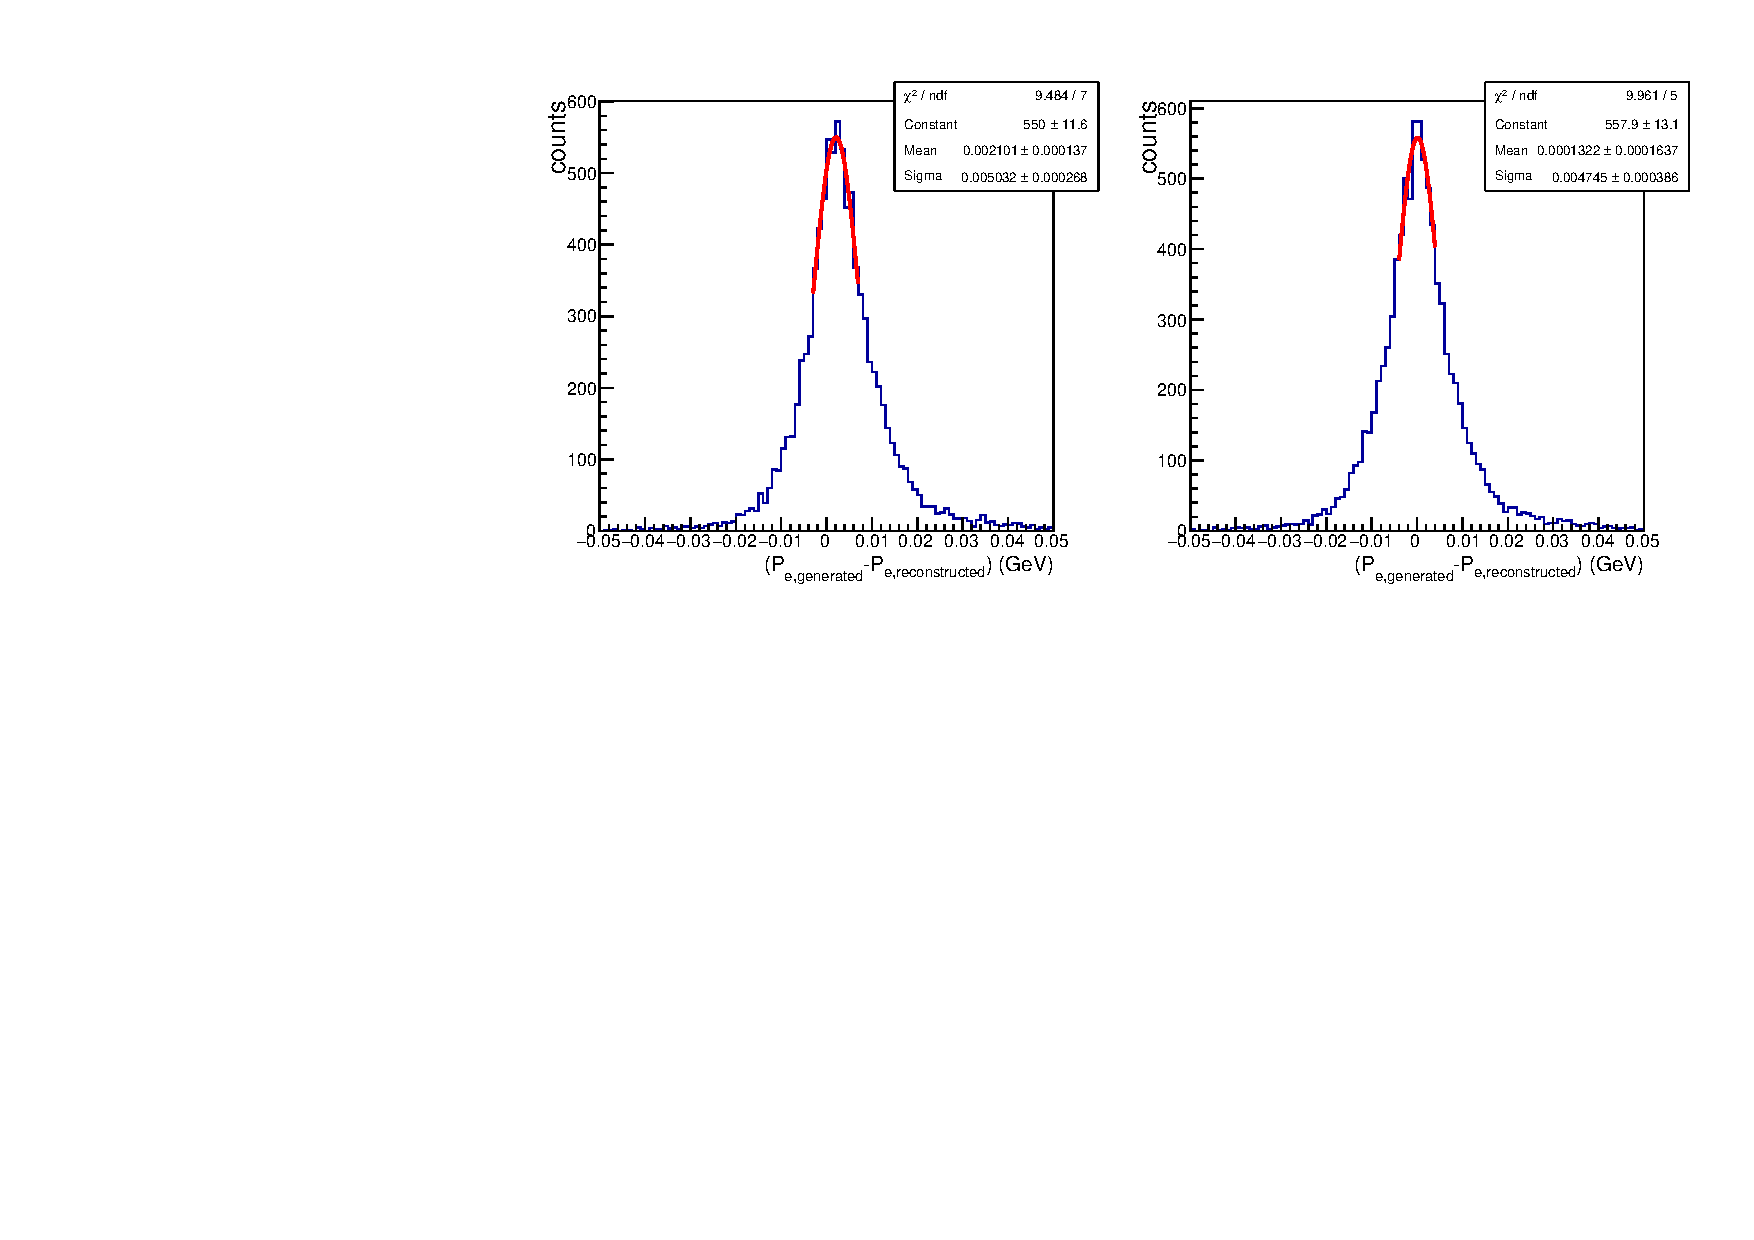
\includegraphics[width=14cm]{pictures/event_selection/mom_corr/el_sim_momcorr/plots/el_sim_mom_corr.pdf}}
\caption{\small The difference between generated and reconstructed electron momenta before (left plot) and after (right plot) the momentum correction has been applied to the reconstructed electrons. \label{fig:el_mom_corr_sim}} 
\end{center}
\end{figure}

\subsection{Proton momentum correction (Energy loss)}
\label{protonmomcor}

While traveling through the detector and the target, the proton loses part of its energy due to interaction with media, hence the measured momentum is lower than the one the proton actually had right after the interaction. This effect is especially important for the low-energy protons and can lead to misdetermination of various kinematical quantities. GSIM simulation of the CLAS detector  correctly propagates protons through the media and is used to account for this effect by using both information about the generated and reconstructed protons. 

To obtain the correction function, event distributions for the differences between generated
and reconstructed proton momenta are binned in proton momentum and proton angle $\theta$ and fit by Gaussians. Then in this way obtained peak positions are fit as function of proton momentum and proton angle $\theta$.
The results are shown in Fig.~\ref{fig:eloss}. The function shown in Fig.~\ref{fig:eloss} gives the percentage of  the momentum that protons lose when they move through the detector and target media.
This function is used to correct the momentum both in the simulation and the data.

It needs to be mentioned that to isolate the pure effect of energy loss, reconstructed events with and without detector and target material need to be compared. Since in the used procedure differences between generated and reconstructed events are analyzed, the correction function shown in Fig.~\ref{fig:eloss} can also include other effects that lead to improper proton momentum reconstruction.

\begin{figure}[htp]
\begin{center}
\framebox{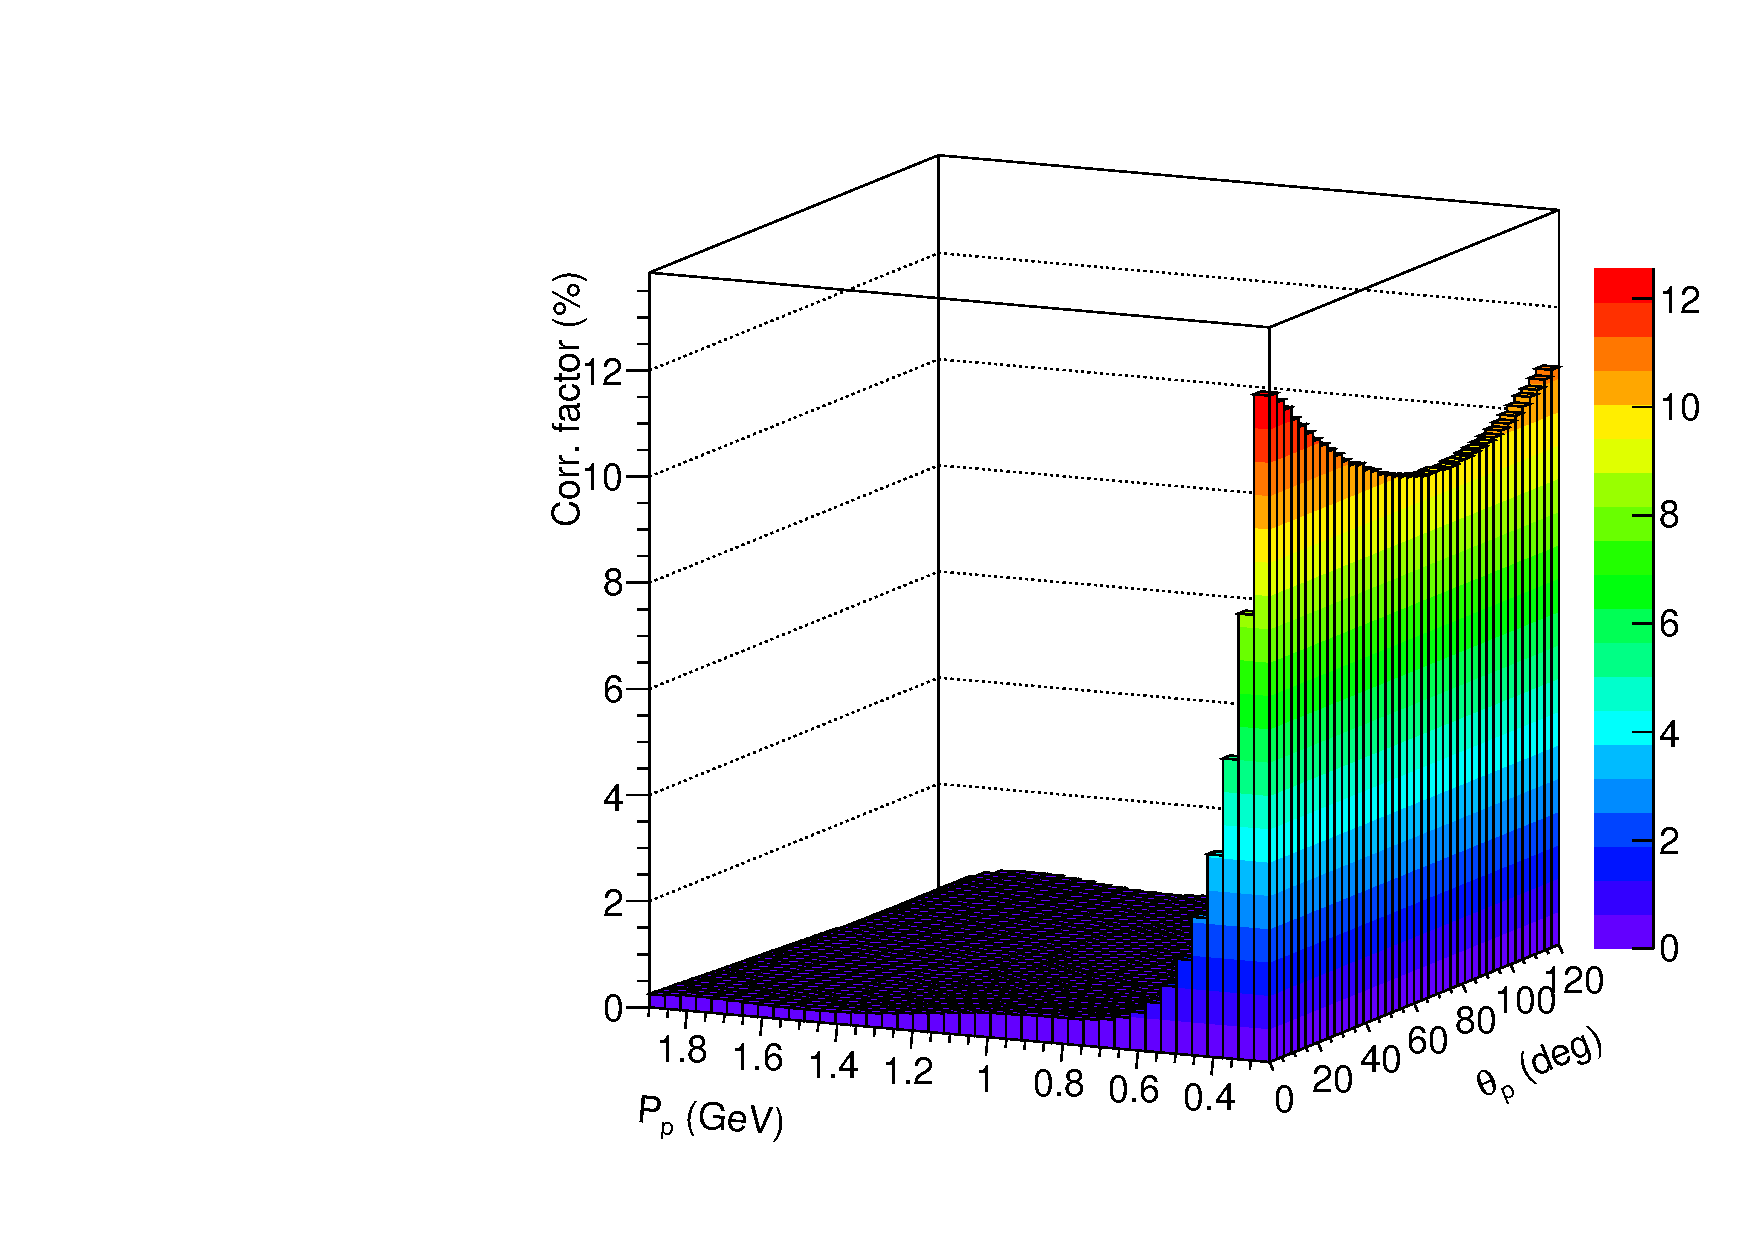
\includegraphics[width=9cm]{pictures/event_selection/mom_corr/proton_eloss/eloss2d.pdf}}
\caption{\small The percentage of momentum that protons lose when they move through the detector and target media as a function of the momentum and scattered angle $\theta$ of the proton. \label{fig:eloss}} 
\end{center}
\end{figure}
